\documentclass{beamer}
\usepackage[utf8]{inputenc}
\usepackage[T1]{fontenc}
\usepackage{lmodern}
\usepackage{tikz}
\usetikzlibrary{math}
\usetikzlibrary{snakes}
\usetikzlibrary{decorations.pathreplacing}
\usepackage[absolute,overlay]{textpos}
\usepackage{booktabs}
\usepackage{ulem}
\usepackage{array}

\title{Abschlusspräsentation}
\author{Projektgruppe FastSense}
\date{11. März 2021}

\usecolortheme{seahorse}
\definecolor{dark}{rgb}{0, 0.1, 0.3}
\definecolor{light}{rgb}{0.9, 0.933, 1}
\definecolor{hw}{rgb}{0.8, 1, 0.9}
\definecolor{sw}{rgb}{0, 0.7, 1}
\definecolor{red}{rgb}{1, 0, 0}
\definecolor{yellow}{rgb}{1, 1, 0}
\definecolor{green}{rgb}{0, 1, 0}
\definecolor{cyan}{rgb}{0, 1, 1}
\definecolor{blue}{rgb}{0, 0, 1}
\definecolor{magenta}{rgb}{1, 0, 1}
\definecolor{grey}{rgb}{0.8, 0.8, 0.8}
\setbeamercolor{normal text}{fg=black}
\setbeamercolor{structure}{fg=dark}
\setbeamercolor{footline}{fg=black}
\setbeamercolor{frametitle}{fg=light,bg=dark}
\setbeamertemplate{itemize items}[circle]
\beamertemplatenavigationsymbolsempty
\addtobeamertemplate{navigation symbols}{}{
    \usebeamerfont{footline}
    \usebeamercolor[fg]{footline}
    {\footnotesize \insertframenumber\\\vspace{0.15cm}}
}
\setbeamertemplate{title page}{
Projektgruppe\\
\vspace{0.2cm}
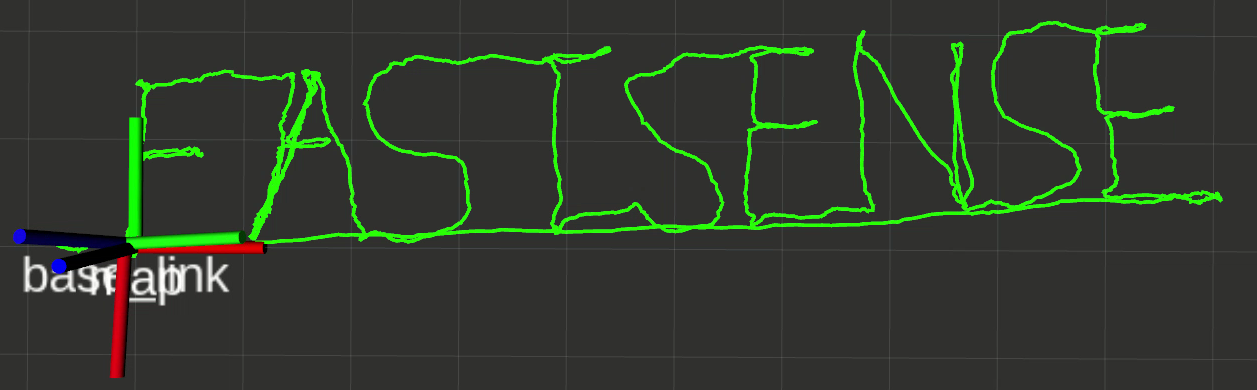
\includegraphics[width=10.8cm]{images/LogoFastSense.png}\\
\vspace{0.5cm}
\begin{LARGE}\textbf{\inserttitle}\end{LARGE}\\
\vspace{0.5cm}
\insertdate
}

\begin{document}

{\setbeamertemplate{navigation symbols}{}
\begin{frame}
\titlepage
\end{frame}}

% \begin{frame}{Inhalt}
% \tableofcontents
% \end{frame}

\section*{Zielsetzung}
\begin{frame}{\secname}
\begin{center}
\begin{tikzpicture}
\node at (-2.5, 5.5) {\begin{minipage}{5cm}\centering
Wissensbasierte Systeme\\
Autonome Robotik\\
\end{minipage}};
\node at (2.5, 5.5) {\begin{minipage}{5cm}\centering
Technische Informatik\\
\end{minipage}};
\node at (-2.5, 4) {
\includegraphics[height=2cm]{images/kbs.png}};
\node at (2.5, 4) {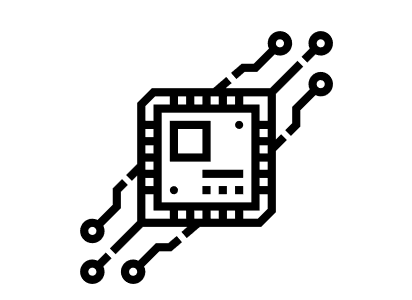
\includegraphics[height=2cm]{images/ti.png}};
\node[below] at (-2.5, 3) {\begin{minipage}{5cm}
\begin{itemize}
\item{SLAM}
\item{TSDF Karten}
\item{LVR2}
\end{itemize}
\end{minipage}};
\node[below] at (2.5, 3) {\begin{minipage}{5cm}
\begin{itemize}
\item{Hardware Beschleunigung}
\item{FPGAs}
\item{High-Level-Synthese}
\end{itemize}
\end{minipage}};
\draw [decorate, decoration={brace, amplitude=0.5cm, mirror}] (-5, 1) -- (5, 1);
\node at (0, 0) {\color{dark}\LARGE\textbf{Hardware Accelerated TSDF SLAM}};
\end{tikzpicture}
\end{center}
% \begin{itemize}
% \item Autonome echtzeitfähige Kartierung
% \item FPGA-basierte Hardwarebeschleunigung
% \item Einfaches, handliches System
% \item Anbindung an bestehende Systeme (LVR2)
% \end{itemize}
\end{frame}

\section{Meilenstein 1}
\begin{frame}
\centering
\color{dark}\LARGE\textbf{\secname}
\end{frame}

\subsection{Vorgehen}
\begin{frame}{\subsecname}
TODO: Bunt, als PDF oder wenigstens weniger verpixelt, evtl Bilder
\begin{center}
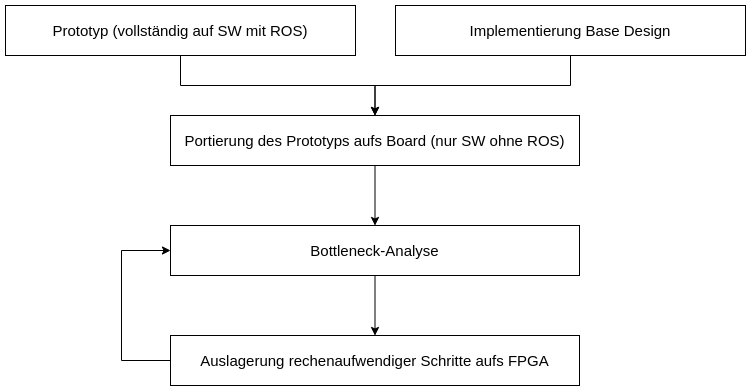
\includegraphics[width=11cm]{images/vorgehen.png}
\end{center}
\end{frame}

\subsection{ReconfROS}
\begin{frame}{\subsecname}
\centering
\begin{tikzpicture}[scale=0.8]
\draw[thick] (-4, 0) rectangle +(2, 5.4);
\node at (-3, 0.5) {\begin{minipage}{2cm}\centering\footnotesize
External\\
ROS Nodes\\
\end{minipage}};

\draw[fill=light] (-3.8, 3.2) rectangle +(1.6, 2) node[pos=0.5] {\begin{minipage}{1.6cm}\centering
%Sensors\\
%\begin{footnotesize}
%Lidar\\
%IMU\\
%Camera\\
%\dots\\
%\end{footnotesize}
\end{minipage}};

\draw[fill=light] (-3.8, 1) rectangle +(1.6, 2) node[pos=0.5] {\begin{minipage}{1.6cm}\centering
%Control\\
%\begin{footnotesize}
%Motor\\
%Battery\\
%\dots\\
%\end{footnotesize}
\end{minipage}};

\draw (0.2, 1.4) rectangle +(6.4, 3.8);
\node at (3.4, 4.9) {\footnotesize Reconfigurable System on Chip};
\node at (3.56, 0.66) {\includegraphics[height=0.96cm]{images/pynq.png}};
\draw (0.2, 1.4) -- (3.1, 0.7);
\draw (6.6, 1.4) -- (3.7, 0.7);
\draw[dark, ultra thick] (3.4, 0.7) circle (0.3);

\draw[fill=light] (0.4, 1.6) rectangle +(2, 3);
\node at (1.4, 4.1) {\footnotesize Processor};
\draw (0.5, 3.1) rectangle +(1.8, 0.5);% node[pos=0.5] {\footnotesize ROS Master};
\draw (0.5, 2.5) rectangle +(1.8, 0.5);% node[pos=0.5] {\tiny Motor Ctrl Node};
\draw (0.5, 1.9) rectangle +(1.8, 0.5);% node[pos=0.5] {\tiny SLAM Node};
%\node at (1.4, 1.75) {\footnotesize \dots};

\draw[shade, left color=light, right color=hw] (2.6, 1.6) rectangle +(1.6, 3);
\node at (3.4, 4.1) {\begin{minipage}{1.6cm}\centering\footnotesize
Shared\\
Memory\\
\end{minipage}};

\draw[fill=hw] (4.4, 1.6) rectangle +(2, 3);
\node at (5.4, 4.1) {\footnotesize FPGA};

\node at (-1, 3.1) {\begin{minipage}{2cm}\centering\footnotesize
ROS\\
Messages\\
\end{minipage}};
\draw[<->] (-2.2, 3.8) -- (0.4, 3.8);
\draw[<->] (-2.2, 2.4) -- (0.4, 2.4);

\draw[thick] (0, 0) rectangle +(6.8, 5.4);
\node[left] at (6.8, 0.3) {\footnotesize ReconfROS};

% Shared Memory
\draw (2.9, 3.15) rectangle +(1, 0.4);
\draw (2.9, 2.55) rectangle +(1, 0.4);
\draw (2.9, 1.95) rectangle +(1, 0.4);

% FPGA
\draw (4.5, 3.1) rectangle +(1.8, 0.5);% node[pos=0.5] {\tiny Path Detection};
\draw (4.5, 2.5) rectangle +(1.8, 0.5);% node[pos=0.5] {\tiny Registration};
\draw (4.5, 1.9) rectangle +(1.8, 0.5);% node[pos=0.5] {\tiny Outlier Removal};
%\node at (5.4, 1.75) {\footnotesize \dots};

\draw[<->] (2.3, 2.75) -- (2.9, 3.35);
\draw[<->] (2.3, 2.15) -- (2.9, 2.75);
\draw[<->] (2.3, 2.15) -- (2.9, 2.15);
\draw[<->] (3.9, 3.35) -- (4.5, 3.35);
\draw[<->] (3.9, 2.75) -- (4.5, 2.75);
\draw[<->] (3.9, 2.15) -- (4.5, 2.15);
\end{tikzpicture}

\vspace{0.3cm}

\begin{tikzpicture}[scale=0.7]
\setlength{\fboxsep}{0pt}
\node[inner sep=0pt] at (0, 5) {\fbox{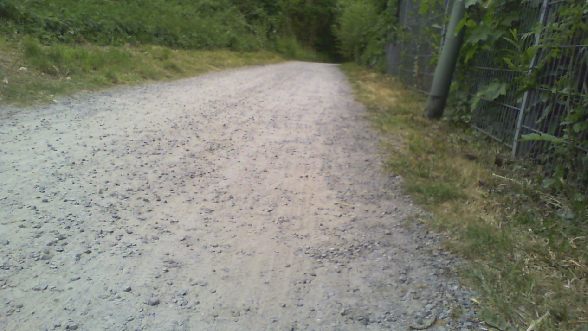
\includegraphics[width=2.1cm]{images/pipeline_pics/cam.png}}};
\node at (0, 3.75) {\footnotesize Camera image};
\node[inner sep=0pt] at (4, 5) {\fbox{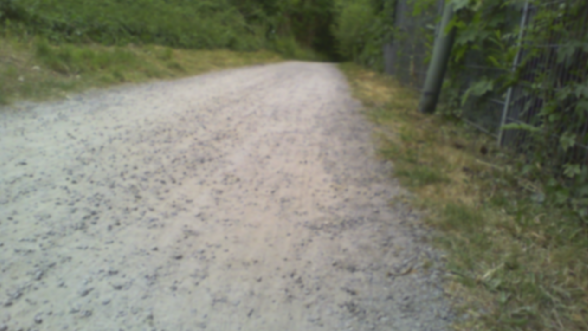
\includegraphics[width=2.1cm]{images/pipeline_pics/gauss.png}}};
\node at (4, 3.75) {\footnotesize Removing noise};
\node[inner sep=0pt] at (8, 5) {\fbox{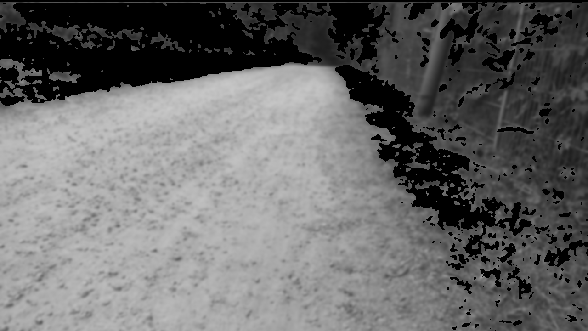
\includegraphics[width=2.1cm]{images/pipeline_pics/green_filter.png}}};
\node at (8, 3.75) {\footnotesize Trail pixel extraction};
\node[inner sep=0pt] at (0, 2) {\fbox{
\includegraphics[width=2.1cm]{images/pipeline_pics/threshold.png}}};
\node at (0, 0.75) {\footnotesize Thresholding};
\node[inner sep=0pt] at (4, 2) {\fbox{
\includegraphics[width=2.1cm]{images/pipeline_pics/morph.png}}};
\node at (4, 0.75) {\footnotesize Remove fragments};
\node[inner sep=0pt] at (8, 2) {\fbox{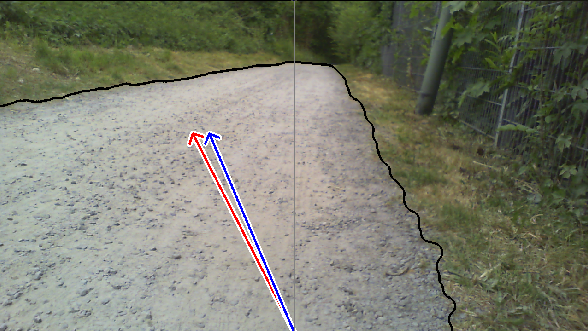
\includegraphics[width=2.1cm]{images/pipeline_pics/direction.png}}};
\node at (8, 0.75) {\footnotesize Trail direction};
\draw[->] (1.5, 5) -- (2.5, 5);
\draw[->] (5.5, 5) -- (6.5, 5);
\draw[->] (9.5, 5) -- (10, 5) -- (10, 3.25) -- (-2, 3.25) -- (-2, 2) -- (-1.5, 2);
\draw[->] (1.5, 2) -- (2.5, 2);
\draw[->] (5.5, 2) -- (6.5, 2);
\end{tikzpicture}
\end{frame}

\section{Meilenstein 2}
\begin{frame}
\centering
\color{dark}\LARGE\textbf{\secname}
\end{frame}

\subsection{SLAM-Box}
\begin{frame}{\subsecname}
\centering
\begin{tikzpicture}
\draw[fill=dark] (0, 0) rectangle +(2, 2) node[pos=0.5] {\color{light}SLAM};
\draw[->] (-1, 1.5) node[left] {Lidar} -- (0, 1.5);
\node at (-3, 2) {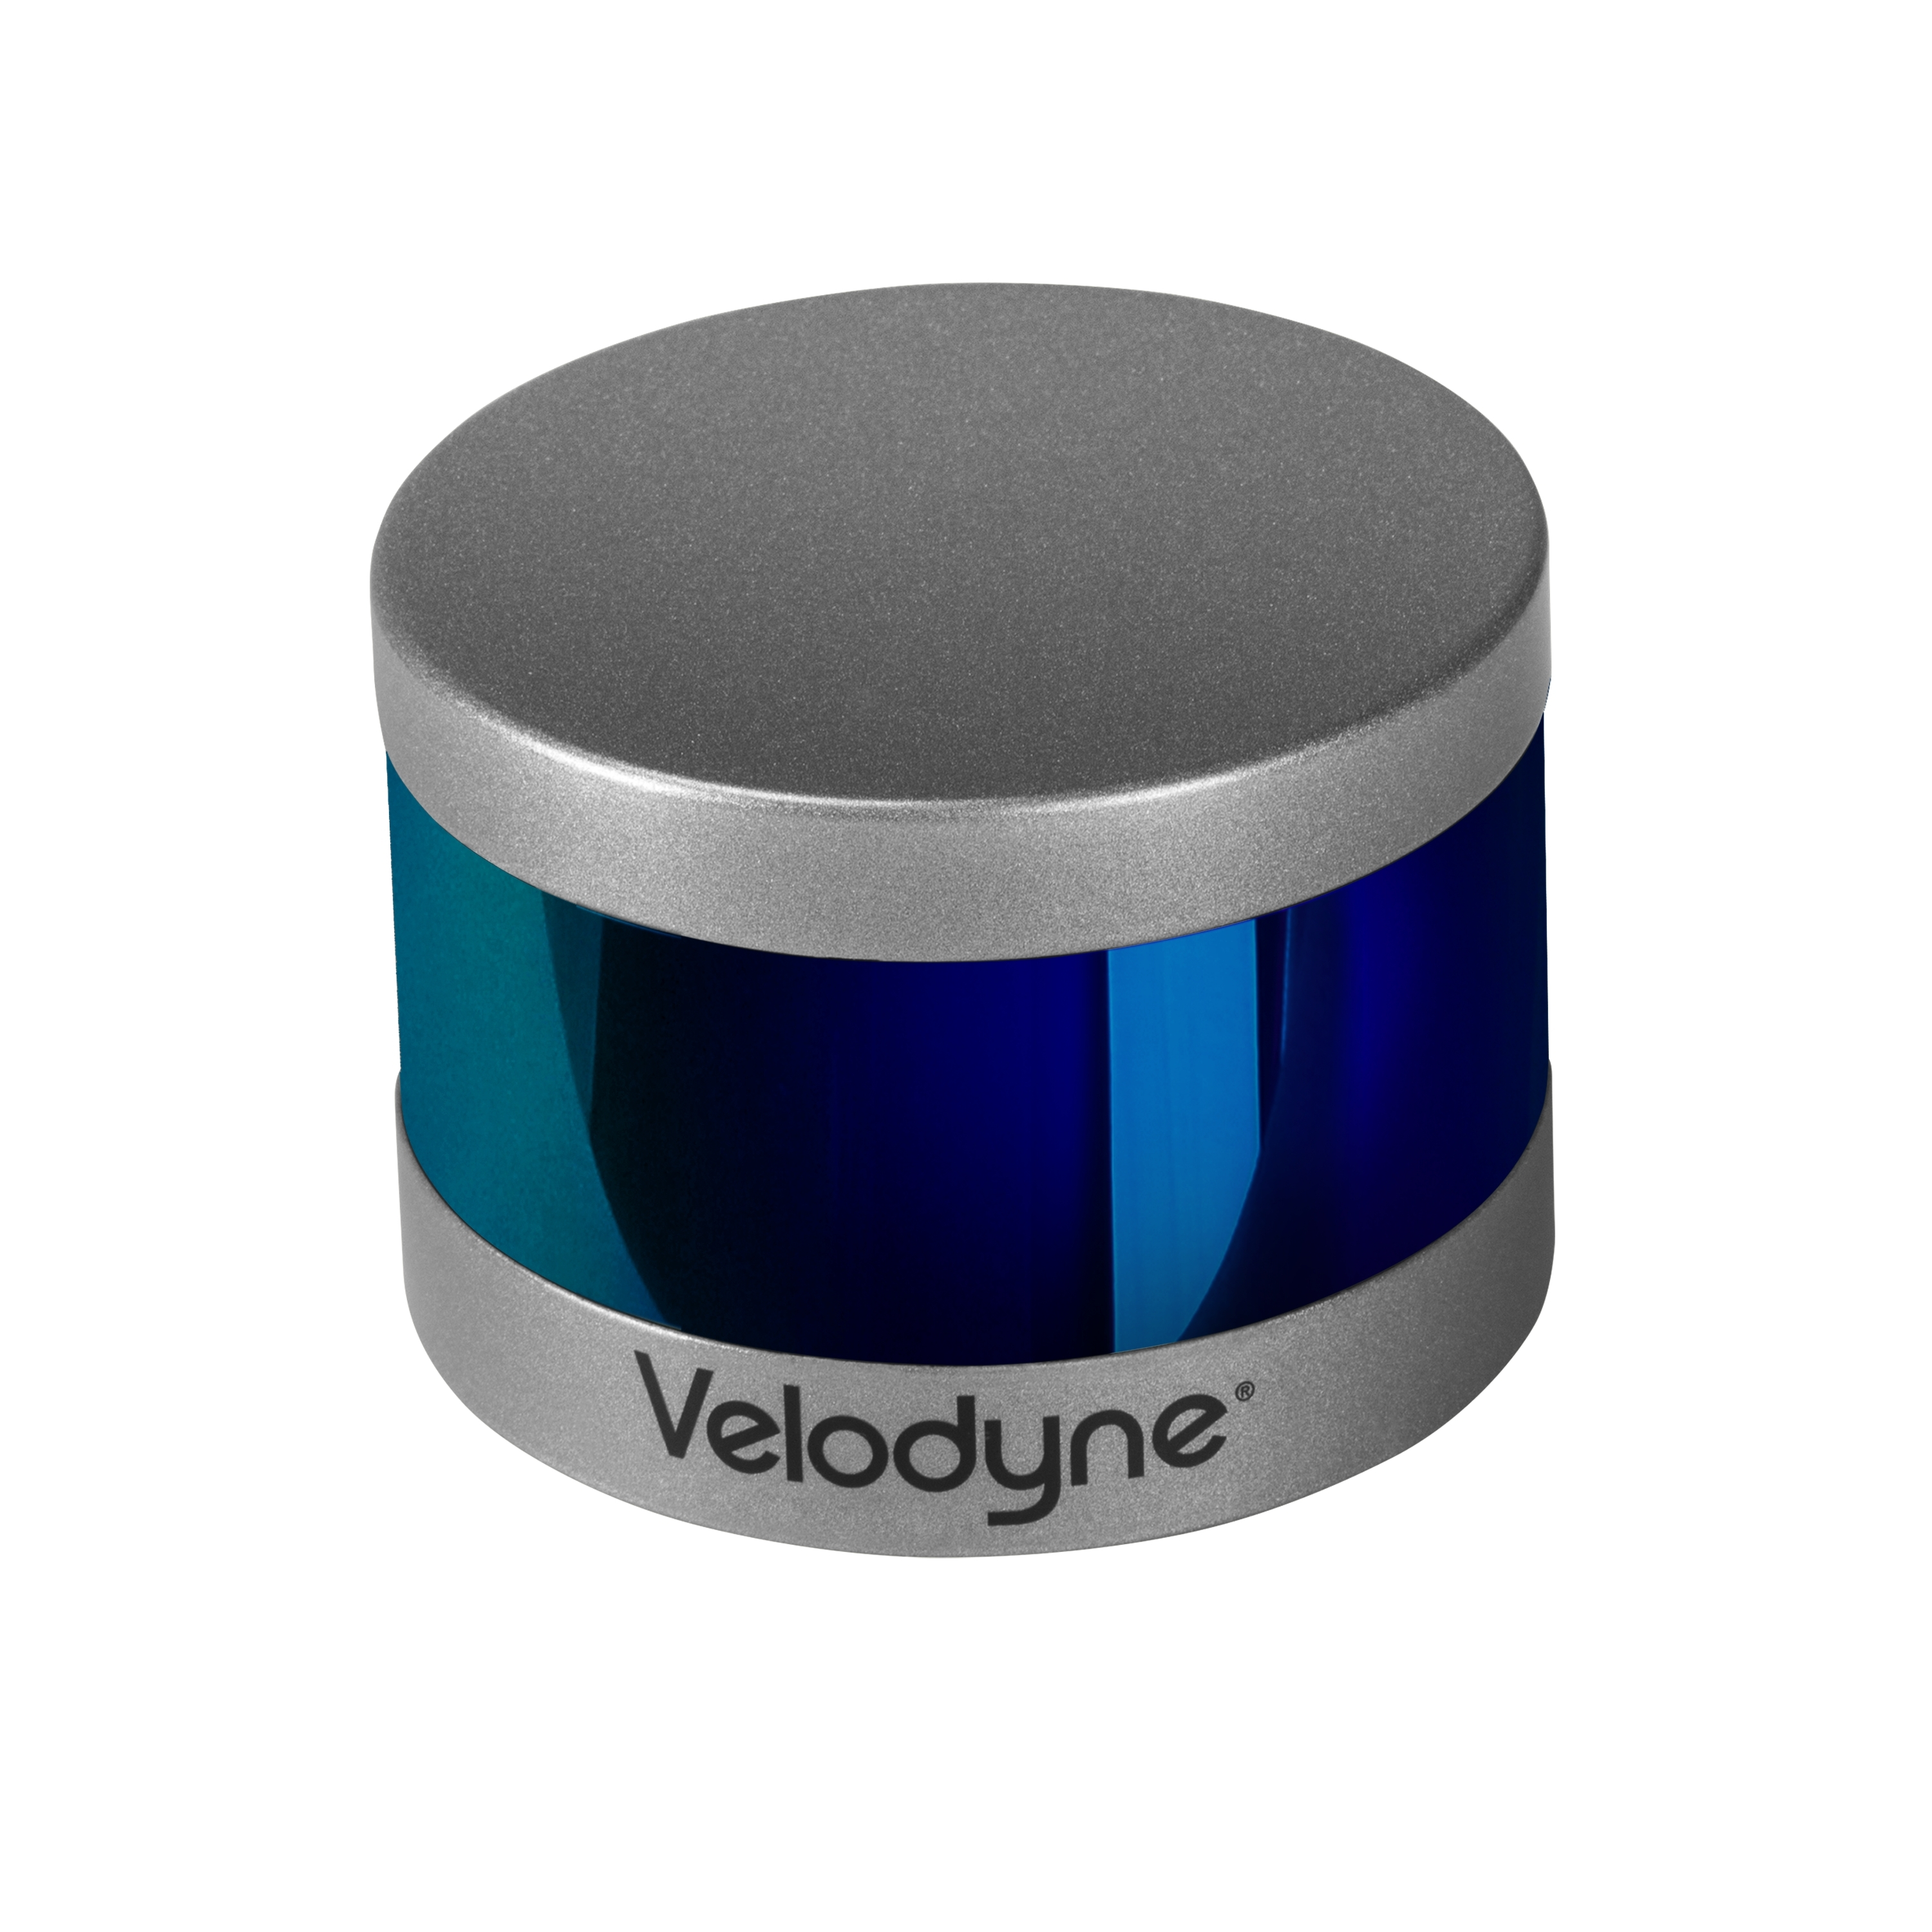
\includegraphics[width=2cm]{images/Velodyne.jpg}};
\draw[->] (-1, 0.5) node[left] {IMU} -- (0, 0.5);
\node at (-3, 0) {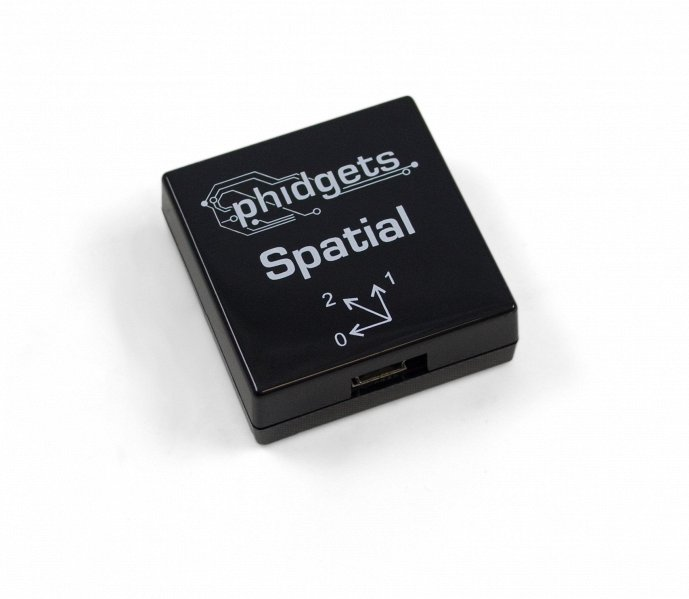
\includegraphics[width=2cm]{images/IMU.jpg}};
\draw[->] (2, 1) -- (3, 1) node[right] {6D Pose};
\draw[red, ultra thick, ->] (5.25, 0.75) -- (6.25, 0.75);
\draw[green, ultra thick, ->] (5.25, 0.75) -- (5.25, 1.75);
\draw[blue, ultra thick, ->] (5.25, 0.75) -- (4.75, 0.25);
\draw[->, dashed] (1, 0) -- (1, -1) node[below] {TSDF Karte};
\end{tikzpicture}
\end{frame}


\section{Vorgehen}
\begin{frame}{\secname}
\begin{center}
\begin{textblock*}{12.8cm}(0cm, 1.8cm)
\centering
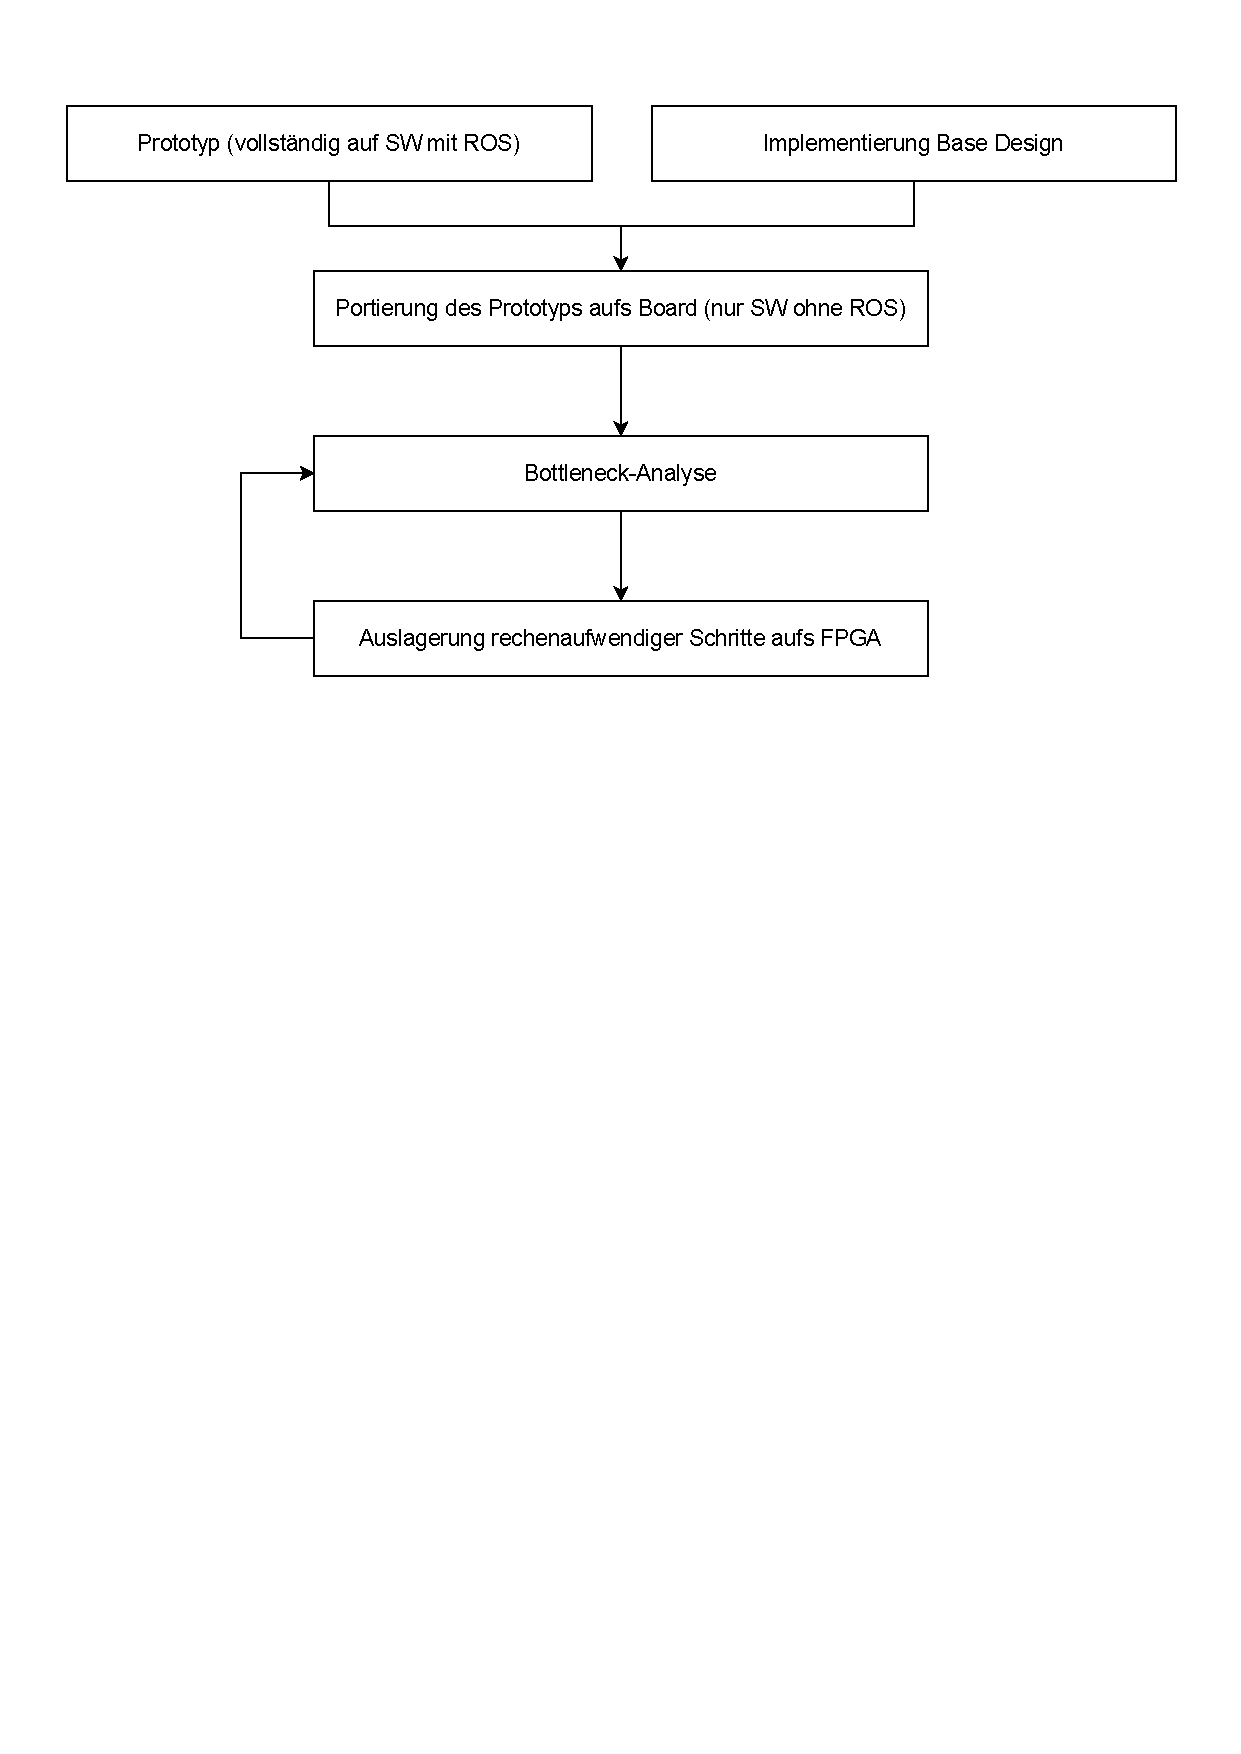
\includegraphics[width=12cm]{images/vorgehen.pdf}
\end{textblock*}
\end{center}
\end{frame}

\subsection{Grundlagen}

\subsubsection*{TSDF}
\begin{frame}{\subsubsecname}
TODO: Bessere Bilder, vllt etwas Text?
\begin{center}
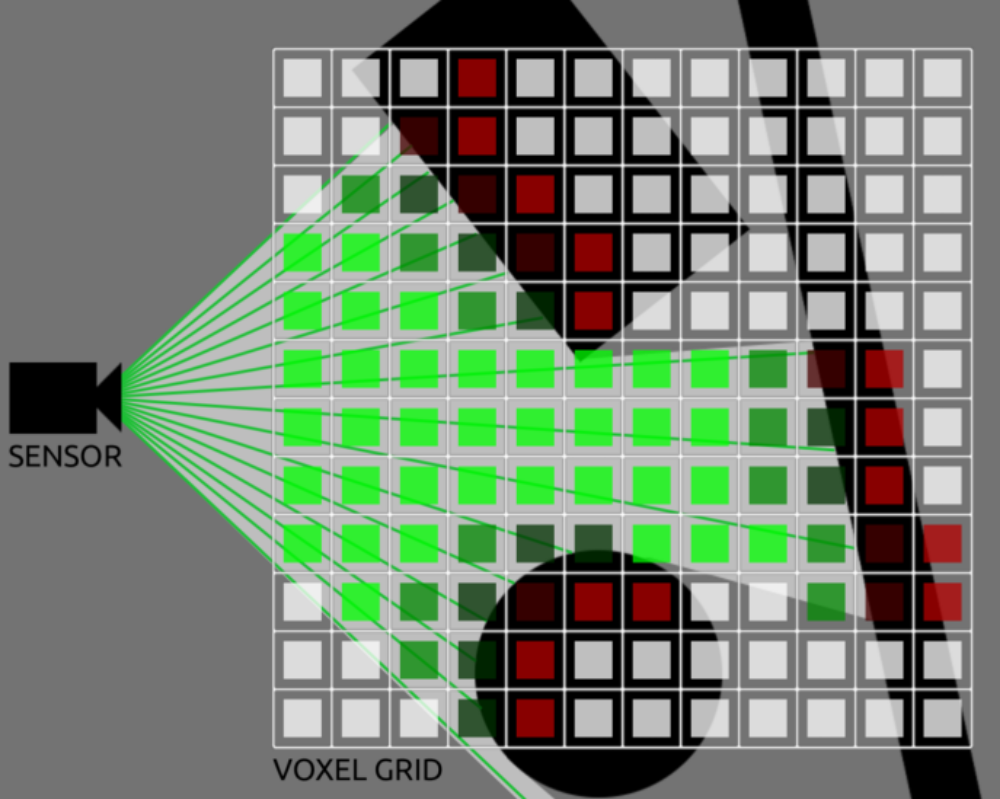
\includegraphics[width=5cm]{images/TSDF_Gen_new.png}
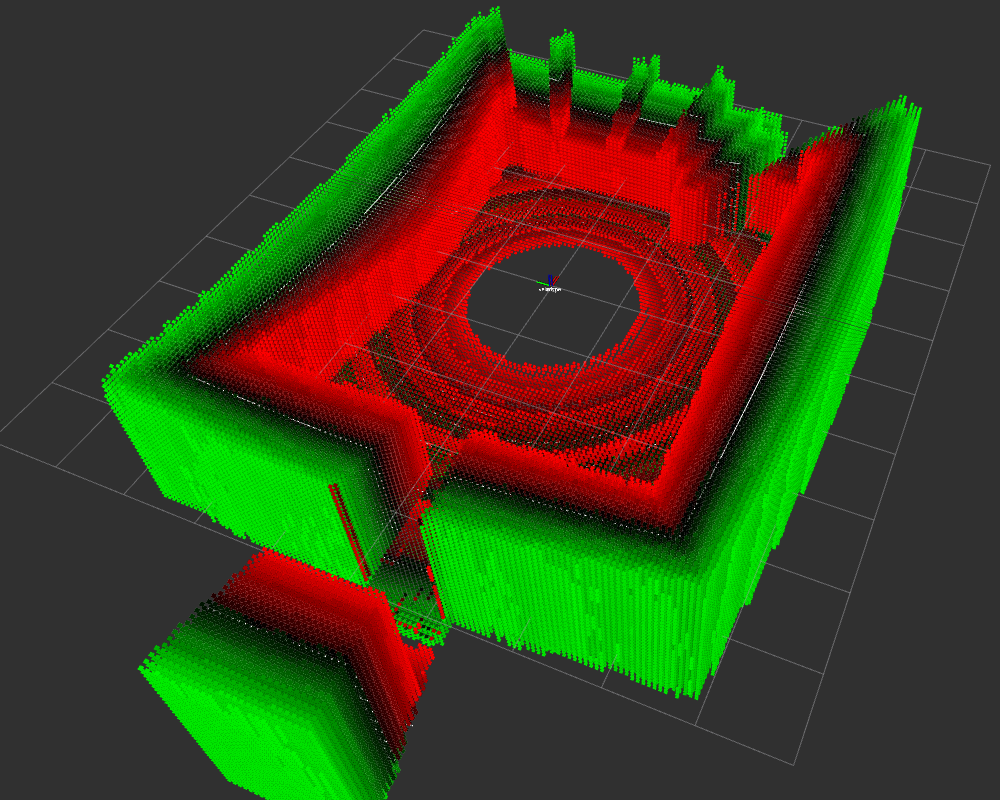
\includegraphics[width=5cm]{images/TSDF_3D.png}
\end{center}
\end{frame}

\subsubsection*{Registrierung}
\begin{frame}{\subsubsecname}
TODO: Bessere Bilder, vllt etwas Text?
\begin{center}
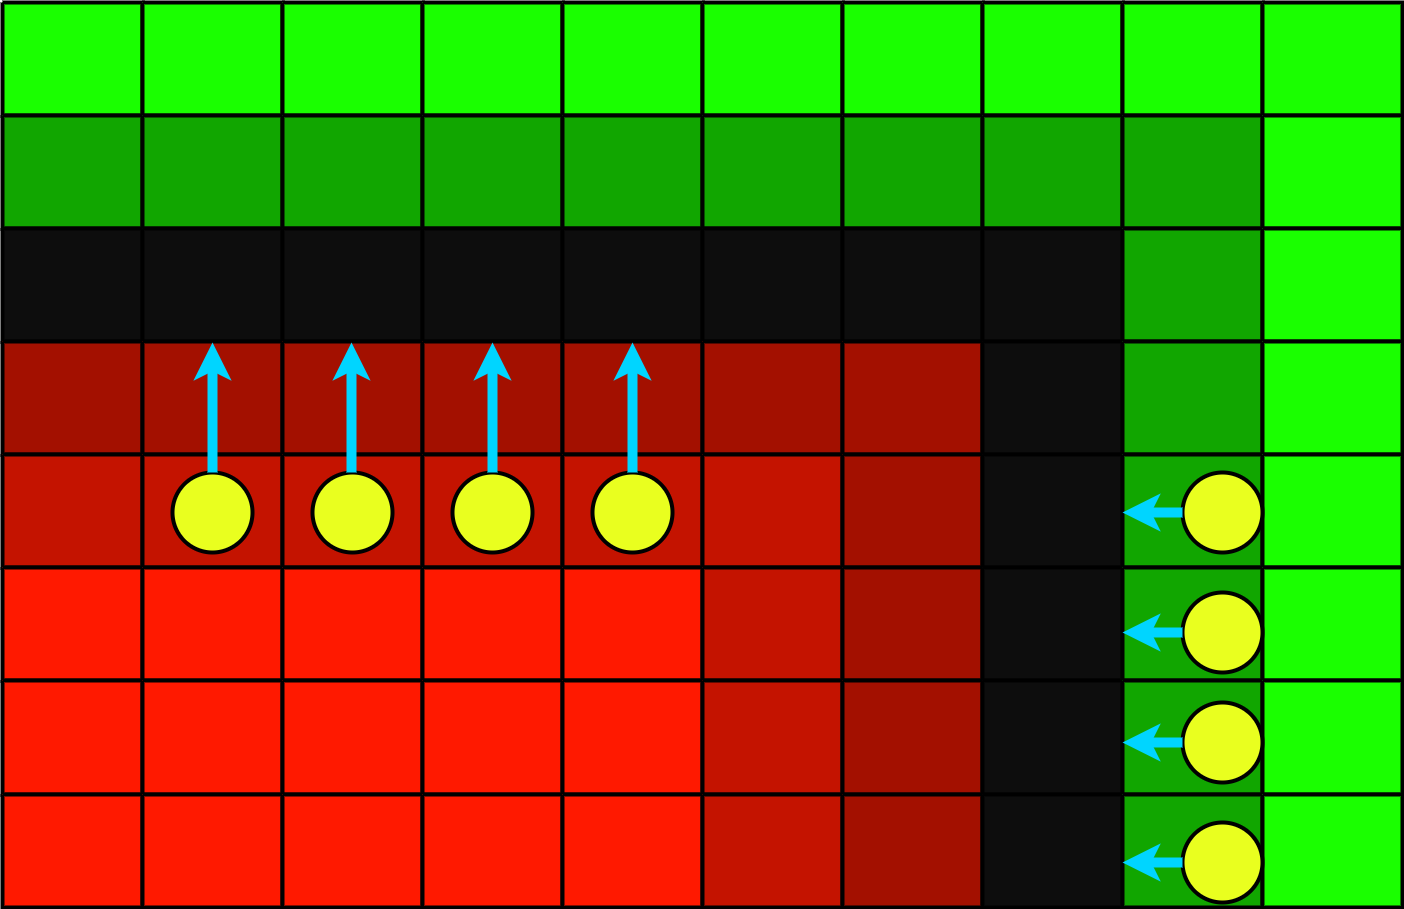
\includegraphics[width=7cm]{images/Reg_Gradient.png}
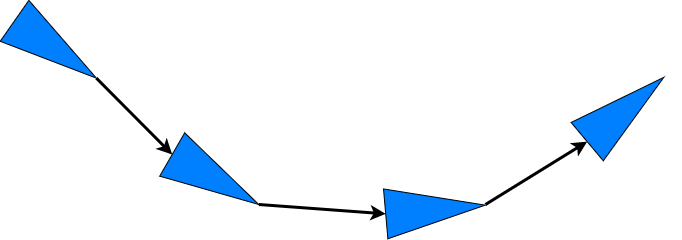
\includegraphics[width=7cm]{images/Pose_Graph.png}
\end{center}
\end{frame}

\section{Meilenstein 3}
\begin{frame}
\centering
\color{dark}\LARGE\textbf{\secname}
\end{frame}

\subsection{Komponenten}
\begin{frame}{\subsecname}
\begin{textblock*}{12.8cm}(0cm, 1cm)
\centering
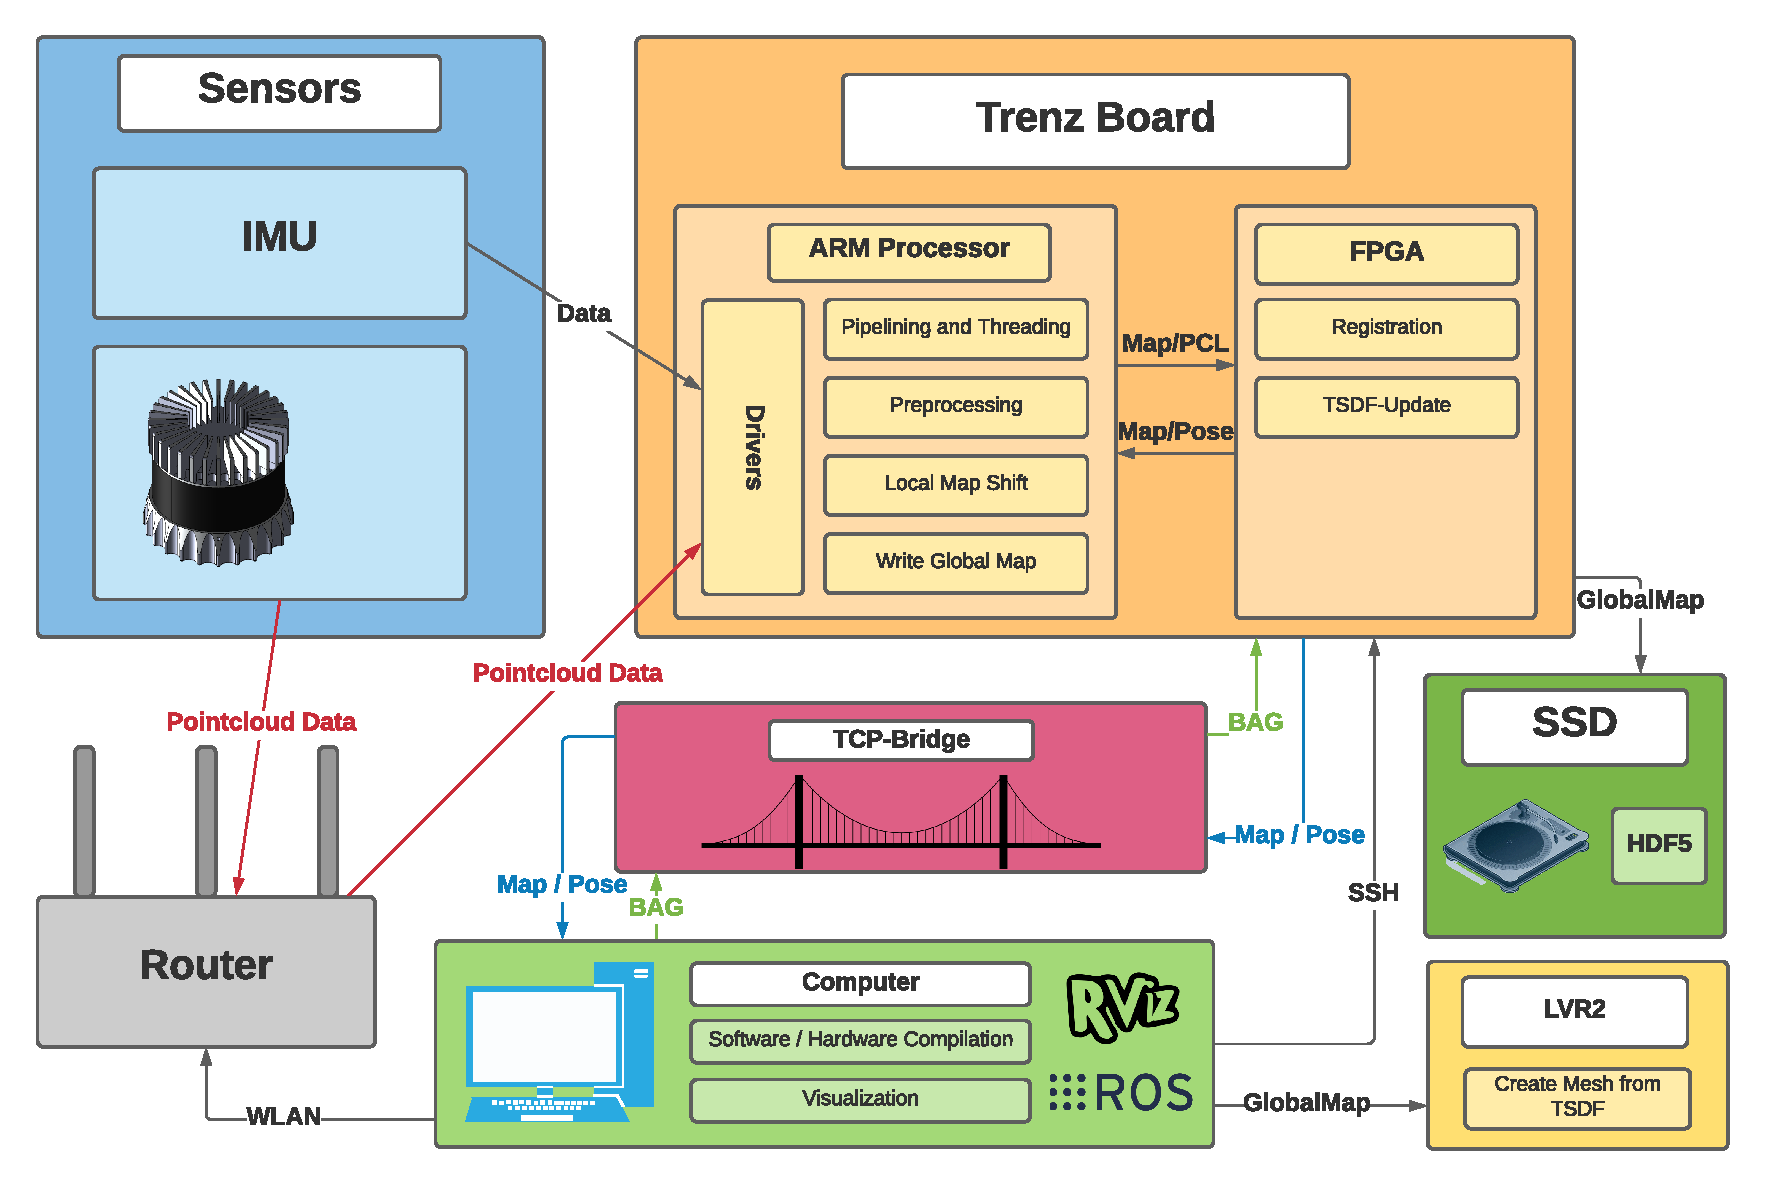
\includegraphics[width=12cm]{images/Architecture.pdf}
\end{textblock*}
\end{frame}

\subsection{Algorithmus}
\begin{frame}{\subsecname}
\begin{textblock*}{12.8cm}(0cm, 1.5cm)
\centering
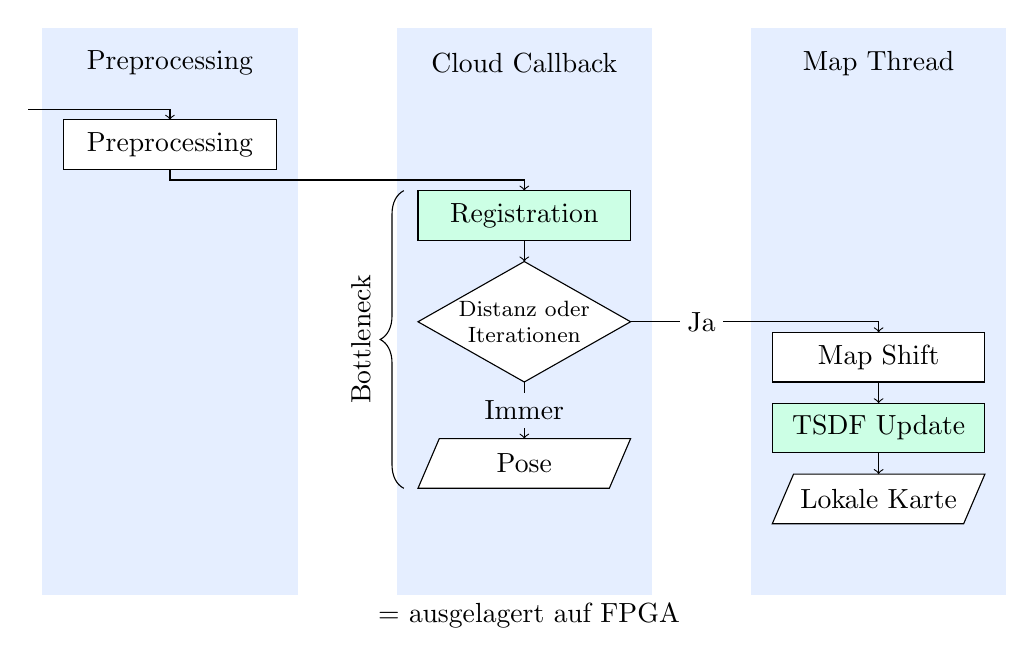
\begin{tikzpicture}[scale=0.9]
\fill[light] (-5.3, 1) rectangle (-1.7, 9);
\fill[light] (-0.3, 1) rectangle (3.3, 9);
\fill[light] (4.7, 1) rectangle (8.3, 9);
\node at (-3.5, 8.5) {Preprocessing};
\node at (1.5, 8.5) {Cloud Callback};
\node at (6.5, 8.5) {Map Thread};
\draw[->] (-5.5, 7.85) -- (-3.5, 7.85) -- (-3.5, 7.7);
\draw[fill=white] (-5, 7) rectangle +(3, 0.7) node[pos=0.5] {Preprocessing};
\draw[->] (1.5, 6) -- (1.5, 5.7);
\draw[fill=hw] (0, 6) rectangle +(3, 0.7) node[pos=0.5] {Registration};
\draw[->] (-3.5, 7) -- (-3.5, 6.85) -- (1.5, 6.85) -- (1.5, 6.7);
\draw[fill=white] (0, 4.85) -- (1.5, 4) -- (3, 4.85) -- (1.5, 5.7) -- cycle;
\node at (1.5, 4.85) {\begin{minipage}{2cm}\centering\footnotesize Distanz oder\\Iterationen\\\end{minipage}};
\draw[->] (1.5, 4) -- (1.5, 3.2) node[midway, fill=light, inner sep=0.1cm] {Immer};
\draw[fill=white] (0, 2.5) -- (2.7, 2.5) -- (3, 3.2) -- (0.3, 3.2) -- cycle;
\node at (1.5, 2.85) {Pose};
\draw[->] (3, 4.85) -- (6.5, 4.85) -- (6.5, 4.7);
\node[fill=white, inner sep=0.1cm] at (4, 4.85) {Ja};
\draw[fill=white] (5, 4) rectangle +(3, 0.7) node[pos=0.5] {Map Shift};
\draw[->] (6.5, 3) -- (6.5, 2.7);
\draw[fill=hw] (5, 3) rectangle +(3, 0.7) node[pos=0.5] {TSDF Update};
\draw[->] (6.5, 4) -- (6.5, 3.7);
\draw[fill=white] (5, 2) -- (7.7, 2) -- (8, 2.7) -- (5.3, 2.7) -- cycle;
\node at (6.5, 2.35) {Lokale Karte};
\draw [decorate, decoration={brace, amplitude=0.3cm, mirror}]
(-0.2, 6.7) -- (-0.2, 2.5) node[midway, xshift=-0.3cm, above, rotate=90] {Bottleneck};
\node at (1.5, 0.7) {{\color{hw}$\blacksquare$} = ausgelagert auf FPGA};
\end{tikzpicture}
\end{textblock*}
\end{frame}

\subsection{Hardware Architektur}
\begin{frame}{\subsecname}
\begin{center}
\begin{textblock*}{12.8cm}(0cm, 1.8cm)
\centering
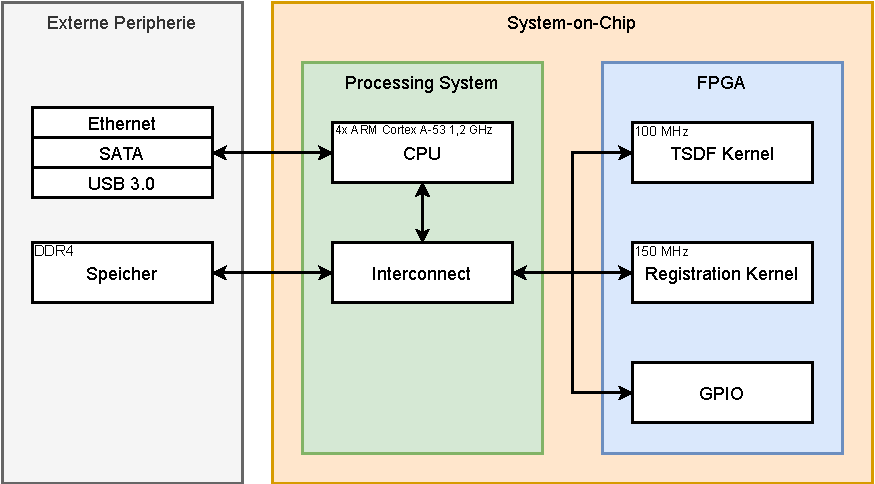
\includegraphics[width=12cm]{images/Blockdiagram.pdf}
\end{textblock*}
\end{center}
\end{frame}

% Kann als Stichpunkt auf die Komponenten Folie

% \subsection{Mesh Rekonstruktion}
% \begin{frame}{\subsecname}
% \begin{itemize}
% \item{Global Map offline}
% \begin{itemize}
% \item{Programm im LVR2 Repository}
% \item{Mesh Verbesserungen}
% \item{HDF5 $\rightarrow$ PLY}
% \end{itemize}
% \item{Local Map online}
% \begin{itemize}
% \item{ROS Node}
% \item{Marker Message $\rightarrow$ Mesh Message}
% \end{itemize}
% \end{itemize}

% \begin{center}
% 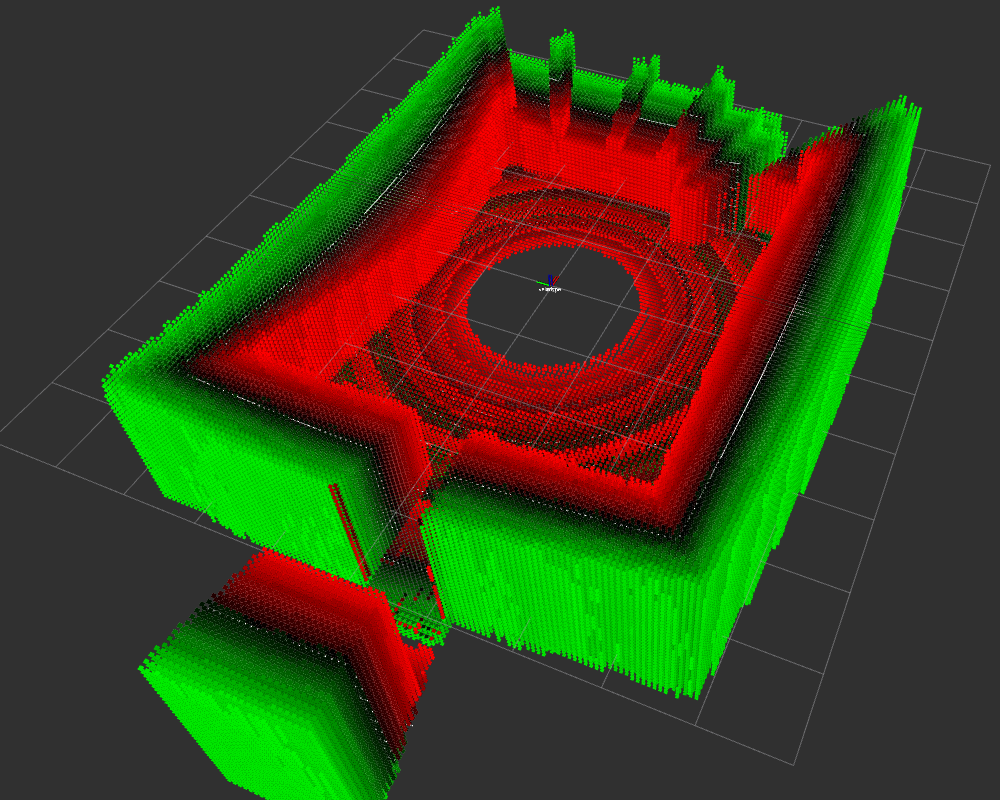
\includegraphics[width=5cm]{images/ReconstructionTSDF.png}
% 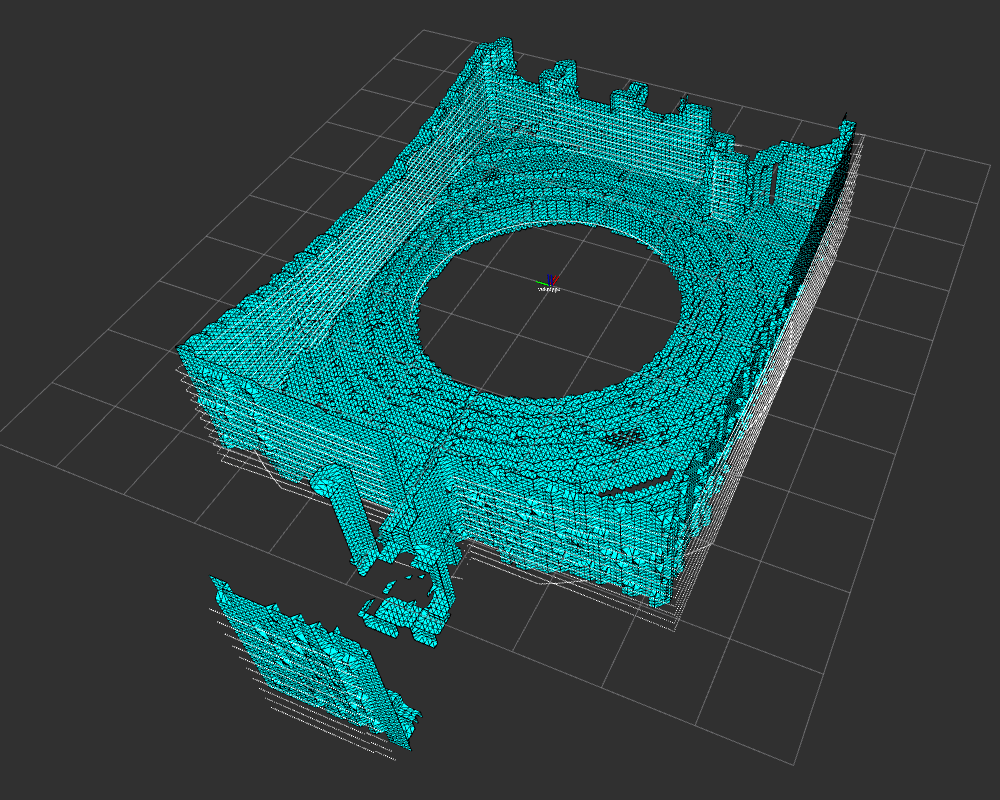
\includegraphics[width=5cm]{images/ReconstructionMesh.png}
% \end{center}
% \end{frame}

\subsection{Aufbau}
\begin{frame}{\subsecname}
\begin{textblock*}{5.8cm}(1cm,1.1cm)
\centering
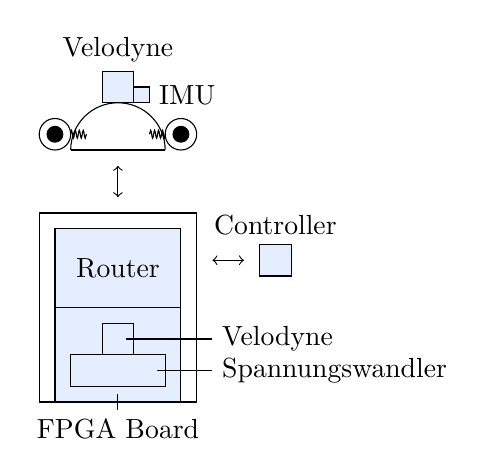
\begin{tikzpicture}[scale=0.4]
\draw (3, 10) arc (0:180:1.5);
\draw (0, 10) -- (3, 10);
\draw[fill=light] (1, 11.5) rectangle +(1, 1);
\node[above] at (1.5, 12.5) {Velodyne};
\draw[fill=light] (2, 11.5) rectangle +(0.5, 0.5);
\node[right] at (2.5, 11.75) {IMU};
\draw [decorate, decoration={snake, segment length=0.5mm, amplitude=0.5mm}]
(0.5, 10.5) -- (-0.5, 10.5);
\draw [fill=white] (-0.5, 10.5) circle (0.5);
\draw [fill=black] (-0.5, 10.5) circle (0.25);
\draw [decorate, decoration={snake, segment length=0.5mm, amplitude=0.5mm}]
(2.5, 10.5) -- (3.5, 10.5);
\draw [fill=white] (3.5, 10.5) circle (0.5);
\draw [fill=black] (3.5, 10.5) circle (0.25);
\draw (-1, 2) rectangle +(5, 6);
\draw[fill=light] (-0.5, 2) rectangle +(4, 3);
\draw (1.5, 2.25) -- (1.5, 1.75) node[below] {FPGA Board};
\draw[fill=light] (1, 3.5) rectangle +(1, 1);
\draw (1.75, 4) -- (4.5, 4) node[right] {Velodyne};
\draw[fill=light] (0, 2.5) rectangle +(3, 1);
\draw (2.75, 3) -- (4.5, 3) node[right] {Spannungswandler};
\draw[fill=light] (-0.5, 5) rectangle +(4, 2.5)
node[pos=0.5] {Router};
\draw[fill=light] (6, 6) rectangle +(1, 1);
\node[above] at (6.5, 7) {Controller};
\draw[<->] (1.5, 8.5) -- (1.5, 9.5);
\draw[<->] (4.5, 6.5) -- (5.5, 6.5);
\end{tikzpicture}
\end{textblock*}
\begin{textblock*}{5.8cm}(1cm,6.7cm)
\centering
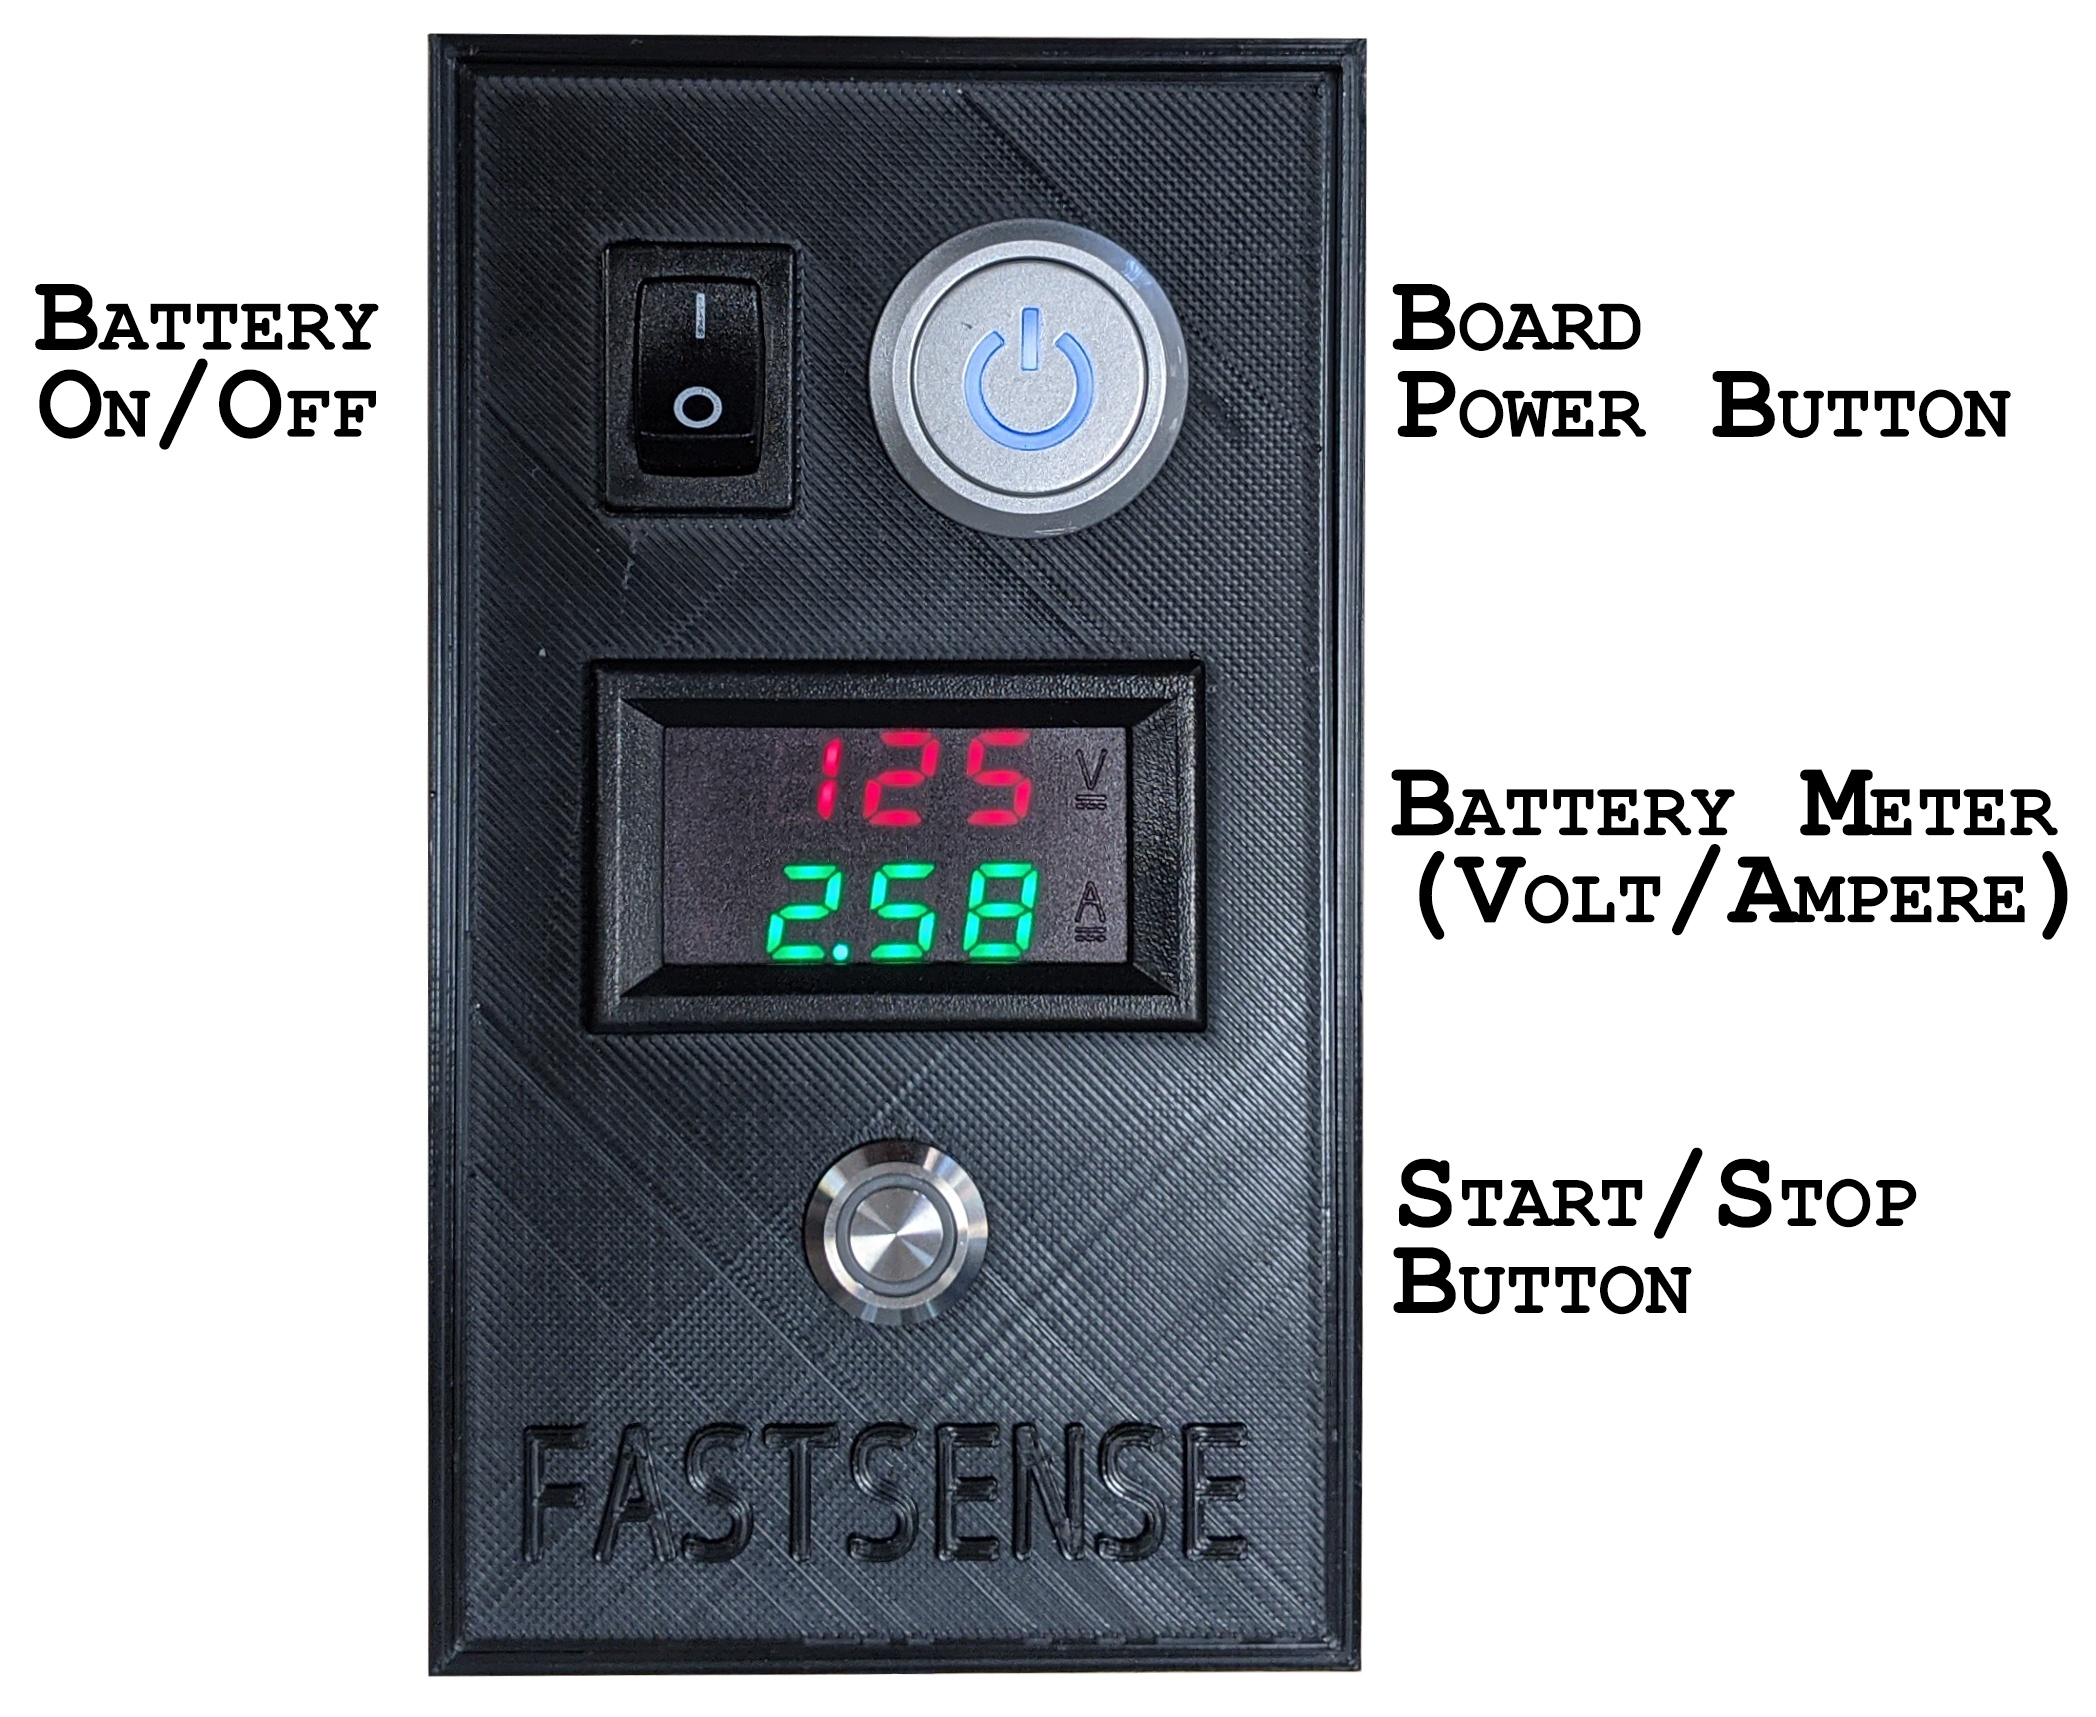
\includegraphics[width=3.5cm]{images/Box.jpg}
\end{textblock*}
\begin{textblock*}{5cm}(6.8cm,1.1cm)
TODO: Alles schicker
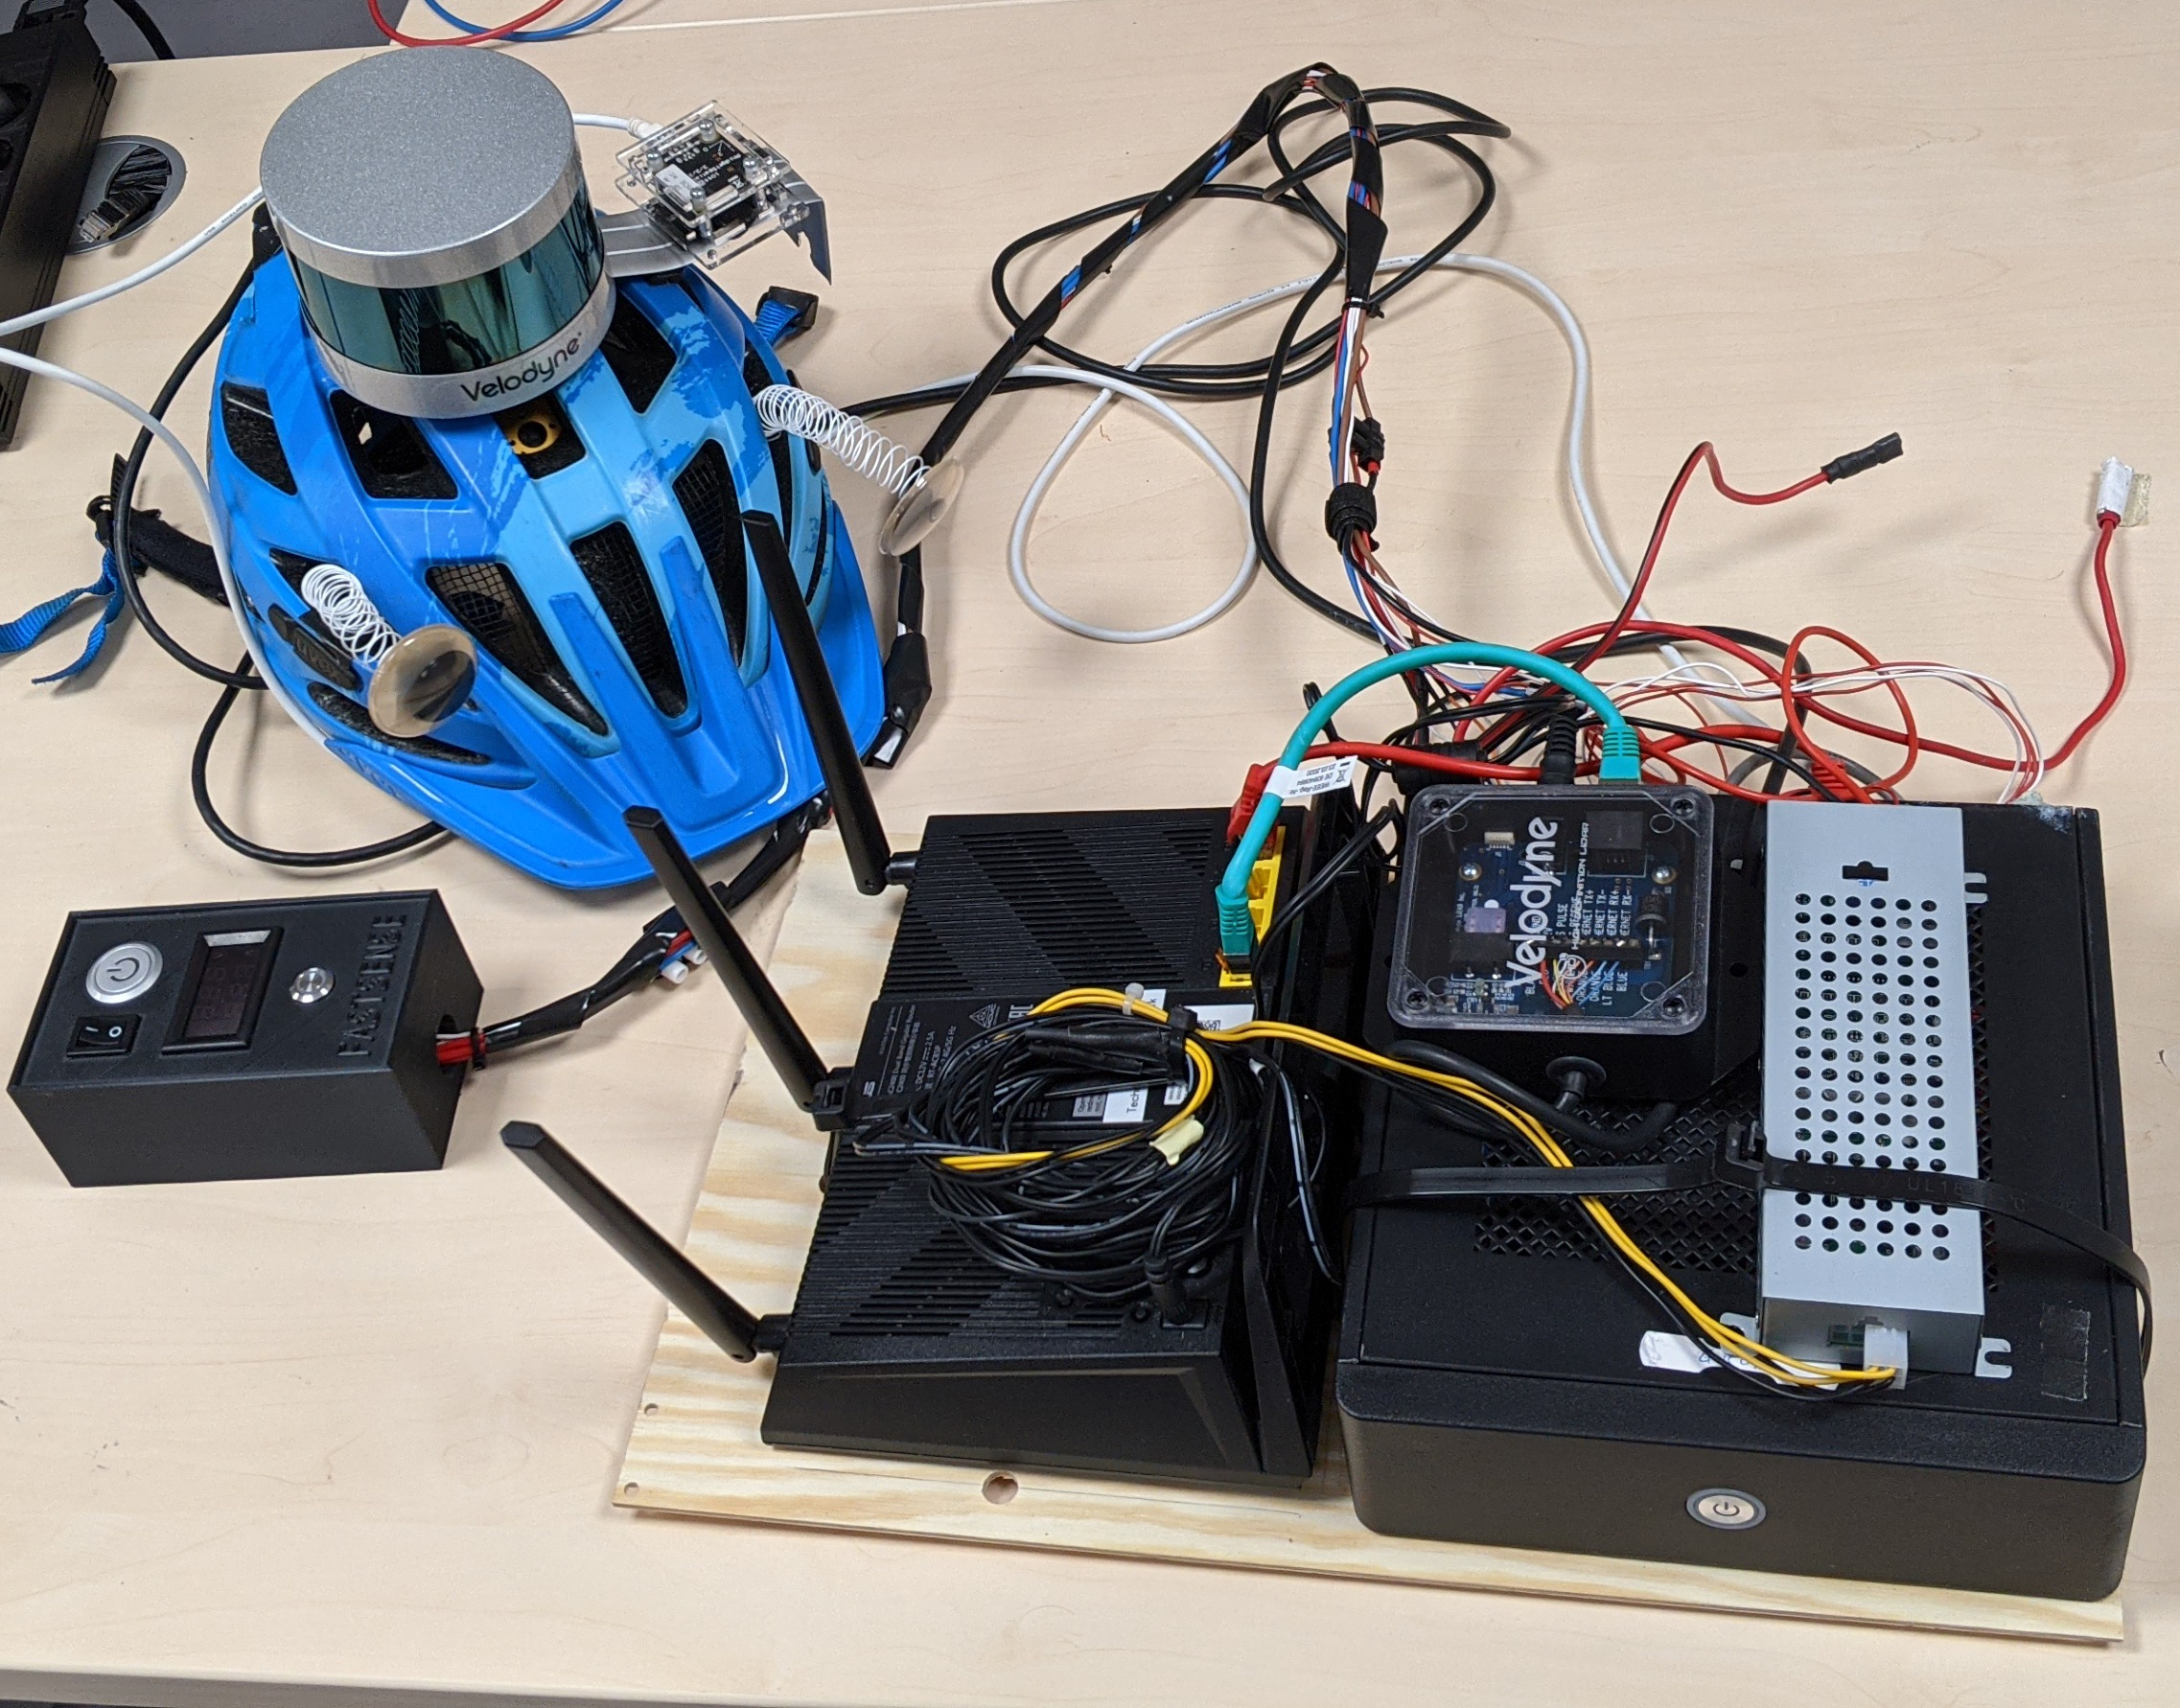
\includegraphics[width=5cm]{images/Rucksack02.jpg}
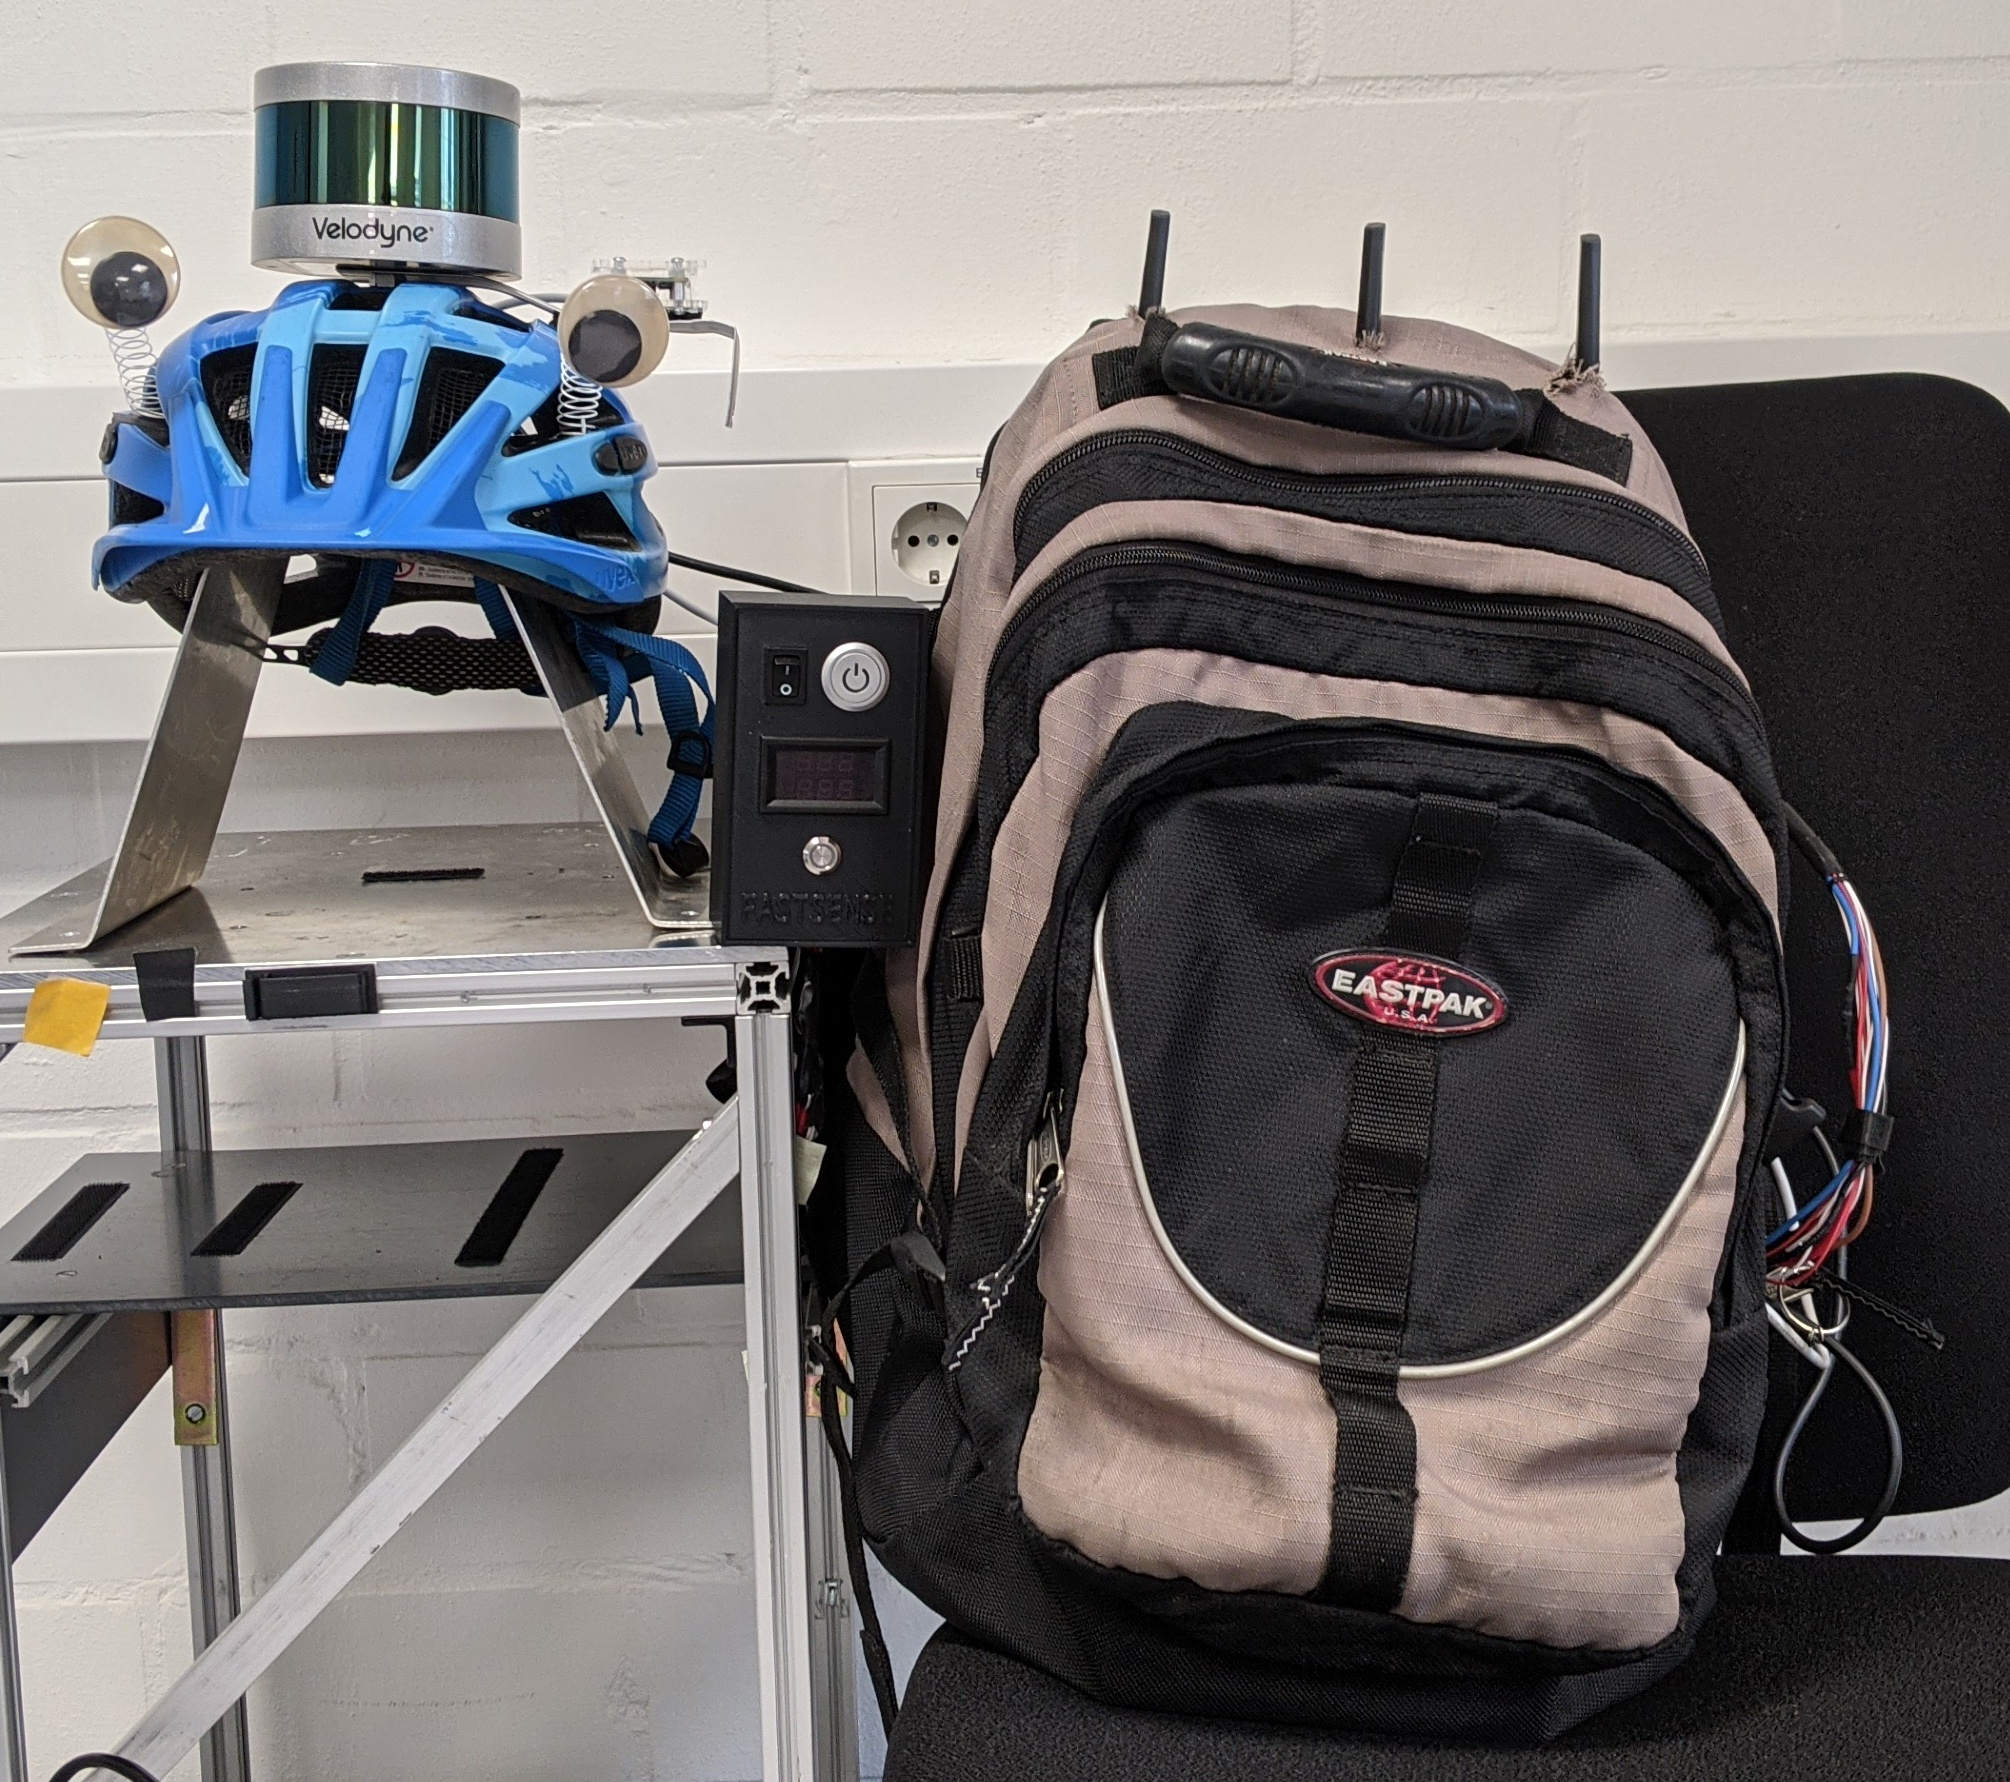
\includegraphics[width=5cm]{images/Rucksack01.jpg}
\end{textblock*}
\end{frame}

\section{Evaluation}
\begin{frame}
\centering
\color{dark}\LARGE\textbf{\secname}
\end{frame}

\subsection{Zeit}
\begin{frame}{\subsecname}
\begin{textblock*}{12.8cm}(0cm, 1.1cm)
TODO
\centering
\definecolor{bad}{rgb}{1, 0.5, 0.4}
\begin{tikzpicture}[scale=0.85]
\draw[->] (0, 0) -- (10.5, 0) node[right] {Zeit [ms]};
\draw[->] (0, 0) -- (0, 8) node[above] {Anzahl Scans};
\foreach \i\y in {0/3,1/11,2/15,3/10,4/7,5/3,6/2,7/1,8/1,9/1} {
    \pgfmathsetmacro\x{int(\i * 10)}
    \draw (\i, -0.1) node[below]{\x} -- (\i, 0.1);
    \tikzmath {
        if {\i < 5} then {
            let \c = light;
        } else {
            let \c = bad;
        };
        { \draw[fill=\c] (\i, 0) rectangle (\i+1, \y/2); };
    }
}
\draw (9.5, 0.25) -- (9.5, -0.5) node[below] {$>90$};
\node[below right] at (6, 8) {\begin{minipage}{6cm}
\begin{itemize}
\item{6. Stock WB; 8000 Scans; \\
$\varepsilon$ = 0,04}
\item{Avg: 30\,ms}
\item[\color{bad}$\bullet$]{11\% aller Scans über 50\,ms}
\item[\color{red}$\bullet$]{2\% gedroppt $\Rightarrow$ 19,6\,fps}
\end{itemize}
\end{minipage}};
\end{tikzpicture}
\end{textblock*}
\end{frame}

% \begin{frame}{\subsecname}
% \begin{textblock*}{12.8cm}(0cm, 1.1cm)
% \centering
% \definecolor{bad}{rgb}{1, 0.5, 0.4}
% \begin{tikzpicture}[scale=0.85]
% \draw[->] (0, 0) -- (10.5, 0) node[right] {Zeit [ms]};
% \draw[->] (0, 0) -- (0, 8) node[above] {Anzahl Scans};
% \foreach \i\y in {0/1,1/5,2/7,3/8,4/8,5/14,6/7,7/3,8/1,9/2} {
    % \pgfmathsetmacro\x{int(\i * 10)}
    % \draw (\i, -0.1) node[below]{\x} -- (\i, 0.1);
    % \tikzmath {
        % if {\i < 5} then {
            % let \c = light;
        % } else {
            % let \c = bad;
        % };
        % { \draw[fill=\c] (\i, 0) rectangle (\i+1, \y/2); };
    % }
% }
% \draw (9.5, 0.25) -- (9.5, -0.5) node[below] {$>90$};
% \node[below right] at (6, 8) {\begin{minipage}{6cm}
% \begin{itemize}
% \item{6. Stock WB; 6000 Scans; \\
% $\varepsilon$ = 0,01}
% \item{Avg: 47\,ms}
% \item[\color{bad}$\bullet$]{48\% aller Scans über 50\,ms}
% \item[\color{red}$\bullet$]{10\% gedroppt $\Rightarrow$ 18\,fps}
% \end{itemize}
% \end{minipage}};
% \end{tikzpicture}
% \end{textblock*}
% \end{frame}    

\subsection{Power Consumption}
\begin{frame}{\subsecname}
\centering
TODO\\
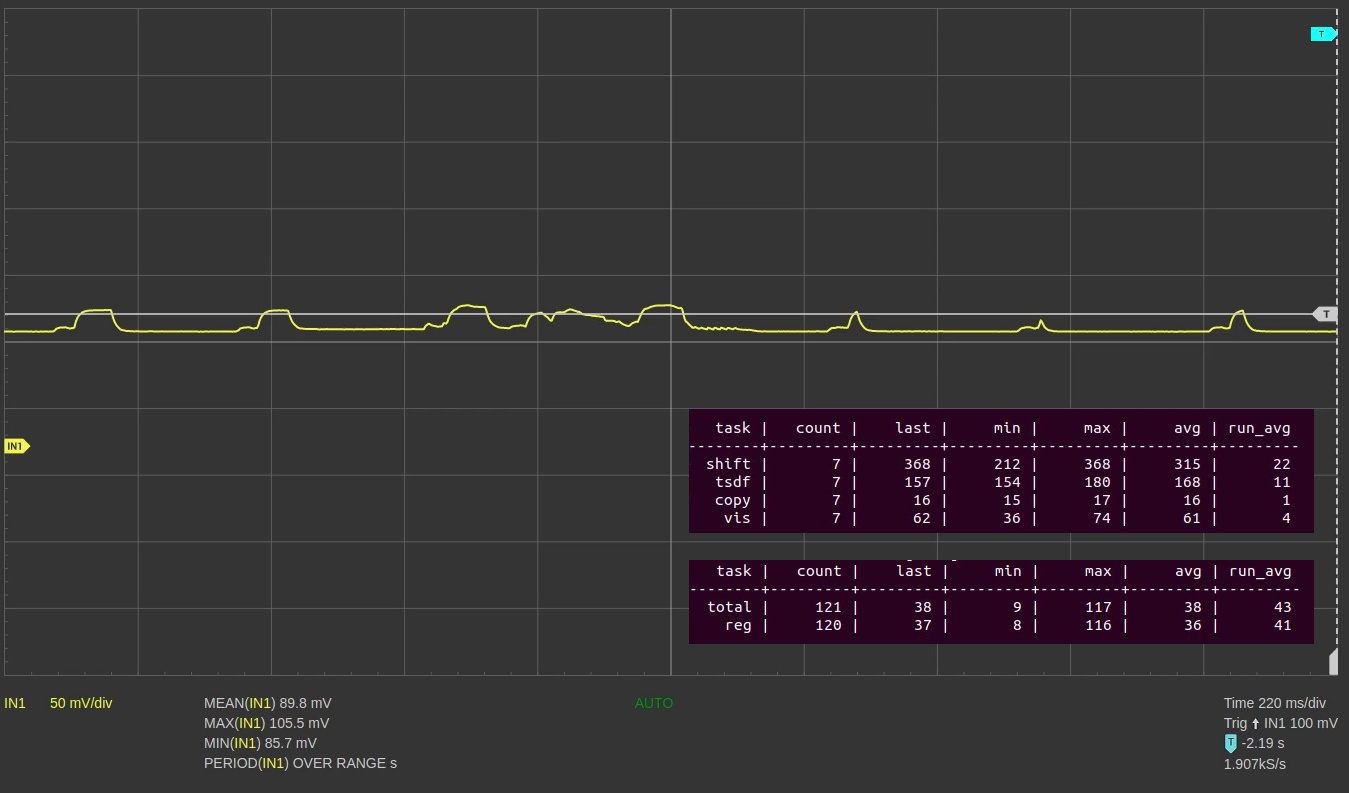
\includegraphics[width=8cm]{images/power_consumption.jpg}\\\vspace{0.5cm}
\begin{tabular}{lllllll}
\toprule
& \multicolumn{3}{c}{Idle} & \multicolumn{3}{c}{Running} \\
& Mean & Min & Max & Mean & Min & Max \\
\midrule
U [mV] & 78,7 & 76 & 88 & 89,8 & 85,7 & 105,5 \\
I [A] & 1,124 & 1,086 & 1,257 & 1,283 & 1,224 & 1,507 \\
P [W] & 13,488 & 13,032 & 15,084 & \textbf{15,396} & 14,688 & 18,084 \\
\bottomrule
\end{tabular}
\end{frame}

\subsection{Genauigkeit}
\begin{frame}{\subsecname}
\begin{itemize}
\item{6. Stockwerk (Distanz in Meter, Auflösung: 6,4\,cm)}
\begin{center}
\begin{tabular}{ccc}
\toprule
$\varepsilon$ & 0,01 & 0,04 \\ 
\midrule
& 0,0615 & 0,0505 \\  
\bottomrule
\end{tabular}
\end{center}
\begin{center}
\begin{tabular}{ccc}
\toprule
Geschw. & langsam & schnell \\ 
\midrule
& 0,0505 & 0,0437 \\  
\bottomrule
\end{tabular}
\end{center}
\begin{itemize}
\item{gesamt (langsam, $\varepsilon$ = 0,04, Strecke $\approx$ \textbf{270m}): 0,075349}
\end{itemize}
\item{8 Meter Labortest (Distanz in Meter, Auflösung: 6,4\,cm)}
\begin{center}
\begin{tabular}{cccc}
\toprule
& hin & zurück & gesamt \\ 
\midrule
langsam & 0,0548 & 0,0650 & 0,0861 \\  
schnell & 0,1676 & 0,0459 & 0,1320 \\
\bottomrule
\end{tabular}
\end{center}
\end{itemize}
\end{frame}

\section*{Fazit}
\begin{frame}{\secname}
TODO
\begin{itemize}
\item{Portables System}
\item{Weiche Echtzeitfähigkeit}
\item{Geringer Stromverbrauch}
\item{Einfache Handhabung}
\item{Einfache Analyse}
\end{itemize}   
\end{frame}

\section*{Ausblick}
\begin{frame}{\secname}
TODO
\begin{itemize}
\item Evaluierung mit anderer Sensorik
\item Portierung auf Drohne
\item Optimierung des Posegraphen (Loop Closing)
\item Paper
\end{itemize}
\end{frame}

\end{document}
